\documentclass{article}
\usepackage[utf8]{inputenc}
\usepackage[left=2.5cm,right=2.5cm,top=2.5cm,bottom=2.5cm]{geometry}

\usepackage{notes2bib}
\usepackage{amsmath}
\usepackage{amssymb}
\usepackage{hyperref}
\usepackage{graphicx}

\usepackage{epstopdf}
\usepackage{epsfig}

\usepackage{paralist} % inline list

\usepackage{amsthm} % theorem and definition
\newtheorem{mydef}{Definition}
\newtheorem{exmp}{Example}

\usepackage{tikz}
\usepackage{xytree}

\usepackage{color}

\usepackage{hhline}
\usepackage{float}
\restylefloat{table}

\title{High-level image interpretation using logical and morphological approaches}
\author{Yifan YANG}

\begin{document}

\maketitle
\section{Introduction}
 High-level semantics extraction from an image is an interesting research area for automatic image understanding in artificial intelligence.
 Many related fields like image annotation, activity recognition and  decision-support systems take advantage of semantic content.
 As advanced as AI has become, it still remains a big challenge for computers to accomplish complex understanding tasks as humans do.
 %However, computers still have difficulties to accomplish complex understanding as humans.  
 Digital image itself is a numerical representation which does not represent explicitly semantic information. 
 Moreover, beyond a single object understanding based on low level features such as colors and forms, we focus on a complex description which relies on context information like spatial relations
 between diverse objects as well as prior knowledge on the application domain.
 For instance, in the context of medical applications, the understanding task can be formulated as giving an abstract description of a pathological brain volume, such as in Figure~\ref{fig:patho_brain}. 
  According to different levels of anatomical prior knowledge on brain pathology, two possible descriptions could be given:
 \begin{itemize}
  \item an abnormal structure is present in the brain,
  \item a peripheral non-enhanced tumor is present in the right hemisphere.
 \end{itemize}
%  according to different prior knowledge of anatomic pathology of the  brain.
%  The second explanation can only be inferred by an experienced doctor with background knowledge.
 In this thesis, a high-level interpretation is regarded as an explanation of what we have seen in the image.
 This process is an inference based on  prior knowledge to link the abstract description and the observed context of the scene.
  \begin{figure}[h]
  \centering
   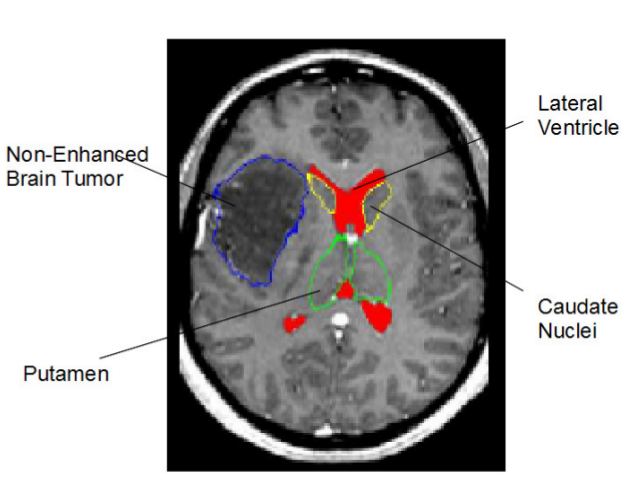
\includegraphics[scale=.2]{./figures/patho_brain.png}
   \caption{\label{fig:patho_brain} A slice of a pathological brain volume (MRI acquisition), where some structures are annotated.}
 \end{figure} 
\subsection{Problem formulation}
According to the objective pointed out in the previous part, the aim is to extract high-level semantic information from a given image and translate it at a linguistic level.
Concretely, we are interested in the interpretation of cerebral images with tumors. The high-level information corresponds to the presence of diverse types of pathologies
 as well as descriptions of brain structures and spatial relations among them in a brain image. 
%  To deal with this problem, prior knowledge at a linguistic level helps the decision making procedure since the semantics is not included in the image.
 In the context of this thesis, the decision process is modeled as an abductive reasoning~\cite{aliseda1997seeking} using a logical formalism, 
 which is an inference mechanism from facts to explanations.
The objective of this thesis is to build a generic logic based formalism as well as  to develop an appropriate reasoning process for image interpretation, 
 allowing us to extract a set of suitable candidates as potential hypotheses for a given image and to select the ``best'' one by a defined criterion.  
%  The knowledge representation is based on an ontology.
 In image interpretation, spatial relationships are important when objects of similar appearance are present in the image, especially in magnetic resonance imaging (MRI).
 Such relationships have then to be included in the representation and in the reasoning process.
  
% In this thesis, a description may not include in the knowledge base and we need to construct it 
% Formal language is a good choice with solid math representation
% First talk about what we need to resolve in this field, which problem, orientations we will take
% Write a general schema here and for each part, what do we have 
  \begin{figure}[h]
  \centering
   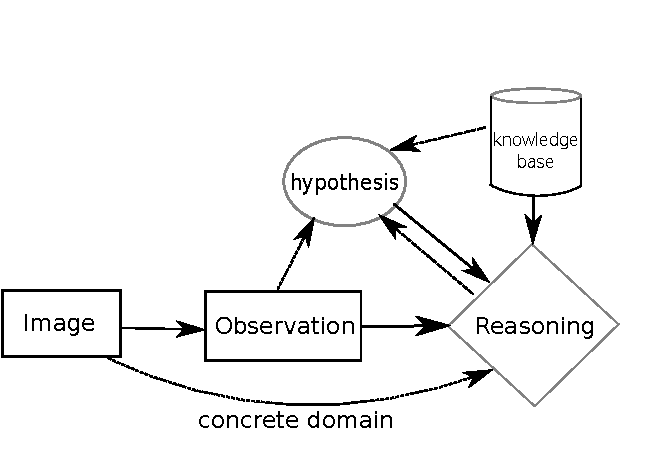
\includegraphics[scale=.8]{./figures/intro_schema.pdf}
   \caption{\label{fig:intro_schema} A general schema of image interpretation task in the thesis.}
 \end{figure} 
Figure~\ref{fig:intro_schema} shows the major components of our framework in this thesis. The given image is translated into symbolic representations in terms of logical form at the beginning.
The image can also serve as the concrete domain in both the knowledge base and the reasoning process. 
Concrete domain is used as a real model to represent abstract terminologies in image space.
A hypothesis of an description might be generated from the observation or the axioms in the knowledge base.
The relations between the hypothesis and reasoning are two directions, which allows validating the hypothesis with the help of standard reasoning and
building a possible hypothesis within non-standard reasoning processes.

To summarize the ongoing and future work, we need to answer the following questions:
\begin{itemize}
 \item \textit{How to model knowledge and formalize an appropriate representation in a given application domain? (Section~\ref{sec:pre})}
 \item \textit{How to connect image level representation and symbolic level representation? (Section~\ref{sec:qsr})}
 \item \textit{How to overcome the semantic gap between numerical representation and qualitative representation of spatial relationships? (Section~\ref{sec:qsr})}
 \item \textit{How to generate hypotheses to explain the observed scene? (Section~\ref{sec:abd} and Section~\ref{sec:persp})}
 \item \textit{How to define a criterion to choose a ``best'' explanation in our case? (Section~\ref{sec:abd} and Section~\ref{sec:persp})}
\end{itemize}
 %  The semantic gap is still an open problem in the field of image interpretation. 
%  This is due to the different level between the numerical measurement in the image and qualitative representation in an expert knowledge.

 \subsection{Related work}
Recognition of perceptual objects and scene understanding, which translate low level signal information into meaningful semantic information, belong to one of the fundamental abilities of human beings.
Semantics is important in image analysis, for various tasks such as image annotation, event detection and diagnostic problems.
In some specific domains, like medical imaging and remote sensing, image interpretation combines image processing with artificial intelligence techniques to derive reasonable semantics.  
Prior knowledge is intensively used by experts who interpret visually an image. Evidently it should then also be used by machines to associate semantics with the image.  
However, image interpretation still faces some difficulties, one of which is how to accurately associate perceptual data with appropriate concepts. Without an expert knowledge,
such a link cannot be established. This relation between visual perception and high-level linguistic expression is called \textit{semantic gap}.


As a high level process of exploiting semantic in the scene, image interpretation involves two levels:
\begin{itemize}
 \item relating low level features to semantics (from pixels to semantic information)~\cite{Bloch2005fuzzy,fouquier2012sequential,Hudelot2008fuzzy,nempont2013constraint}.
 \item inferring the description from the semantic image content (from semantics to explanation)~\cite{atif2014explanatory,Espinosa07multimedia}.
\end{itemize}

Roughly speaking, the first level describes what is happening while the second one describes how it is happening~\cite{tsotsos1992image}.
The first level has been mainly studied in the field of multiple objects recognition. 
Image interpretation maps regions or groups of regions onto labels corresponding to semantic concepts (e.g. labels of anatomical structures for medical images).
Various approaches employ Bayesian networks with a combination of semantics and probabilistic inference mechanisms~\cite{Luo2005Bayesian,Niko2009evidence,Singhal2003proba}.
These techniques provide inference mechanisms by attempting to construct co-occurrence objects and contextual information with a probabilistic model for reasoning.

Further, a hierarchical representation of knowledge base is proposed, called image grammar~\cite{tu2014joint,zhu2006stochastic}. The grammar is a structured knowledge represented by an And-Or graph.
In this graph, a global description of a scene is decomposed into parts, objects until primitive pixel patches from top to bottom.
An And-node consists of a set of successive components and an Or-node is composed by alternative nodes.
A parsing method is proposed as inference within a probabilistic model in each node~\cite{han2009bottom,wu2011numerical}. 

The second level consists in reasoning at the language (knowledge) level.
For the purpose of giving an adequate explanation, the second level is a logic-based reasoning to depict the image with a deep and abstract description from the point of view of an expert.
There is not much work on image interpretation using logical knowledge representation and reasoning. 
However, formal language based on logic formalism has  strong associated semantics for knowledge representation as well as reasoning processes. 
An aggregation concept is proposed in~\cite{Espinosa07multimedia} to represent a complex event or scene concerning occurrence objects, as well as spatial and temporal constraints configuration.
According to these defined aggregation and specific rules, a high-level interpretation is able to be inferred~\cite{neumann2008scene}.
In addition, the results using Bayesian networks and image grammars are limited to defined descriptions.
A complex description can also be generated when non-explicitly presented in the knowledge base~\cite{atif2014explanatory}.

% Because the Bayesian network and image grammar method are  

%  Since a large number use of multimedia in daily life, semantic information extraction of images has been variously studied in many fields such as image annotation, event detection and diagnostic problems.
%  These areas involve different methodologies like machine learning . Many work 
% Image interpretation based on knowledge representation


% What knowledge is needed for image interpretation?
% How to represent it?
% Formal language
% How to produce an inference to get the result?
% 
%  We need to interpret it with prior knowledge.
%  In this thesis, we focuses on diagnostic problem (decision support system) in LOGIMA project
%  The knowledge may not be accurate presented and correspond what we are looking at. Lack of expressivity graph representations.
% 
% The context and  main objective of my thesis will be developed in this part.
% I would like to present a short bibliography of image interpretation. Then, I would like to present
% that we focus on diagnostic problem and we treat this problem as an abductive reasoning with a knowledge base represented by description logics.
% I also explain the reason why we choose this kind of method (its advantages).

\section{Preliminaries}\label{sec:pre}
\subsection{Ontology}
Experts' knowledge is expressed in terms of diverse vocabulary of special domain in natural language which is difficult to be interpreted by machines.
In order to facilitate an automated reasoning process with a background knowledge base, a structural semantic based model is  an effective means to represent prior knowledge.
The term ontology is derived from philosophy and then used for the purpose of expressing common sense knowledge in computer science~\cite{alexander1986knowledge}.
Since then, ontologies were adopted for image interpretation tasks~\cite{bannour2011towards,Hudelot2008fuzzy,town2006ontological}.
Ontologies are defined as “\textit{a formal specification of a shared conceptualization}"~\cite{studer1998knowledge},
which deal with modeling a universal and reusable knowledge among different applications for a specific domain.
Ontologies were also studied for reasoning service within its expressive formal description. 
An ontology mainly contains  \textit{individuals}, \textit{concepts}, \textit{properties} and \textit{axiom rules}. 
These components enable the background knowledge to be understood and processable by machines.

\subsection{Description Logics}
As mentioned above, ontologies require a formal representation language and well-defined semantics for reasoning services. 
Description Logics (DLs) is a family of knowledge representation logical formalisms, which is seen as good candidates for ontologies~\cite{horrocks1999description}.
The basic elements of Description logics are concepts (unary predicates), roles (binary predicates) and individuals.
Besides the formal knowledge representation, another important feature of DLs is their ability of reasoning.
% the other reason of treating DLs as an important logical formalism is its ability of reasoning process.
Implicit information can be inferred from explicit knowledge description, such as satisfiability checking~\cite{baader2003description}. 
In this part, we introduce syntax and semantics of a description logic language $\mathcal{ALC}$ as well as its reasoning services.
\subsubsection{Syntax and semantics}
We first recall the syntax and semantics of the basic language of Description Logics ($\mathcal{ALC}$) ~\cite{baader2003description}.
\begin{mydef}[Signature]
 The syntax of a Description Logic is defined over a signature, which is defined as three disjoint sets $Sig~=~(N_C,~N_R,~N_I)$. $N_C$ is a set of concept names that refers to a set of entities
 with the same characteristics. $N_I$ is a set of individuals that contains instances of the concepts in $N_C$.  $N_R$ is a set of role names that refers to the binary relationships between 
 two individuals or two concepts.
\end{mydef}


\begin{mydef}[Concept expression]
 The set of concept expression is recursively built from the signature as follows:
 \begin{itemize}
  \item all the concept names, as well as $\top$ (top concept) and $\bot$ (bottom concept) are concepts,
  \item if $C$ and $D$ are two concepts in $N_C$ and $r$ is a role in $N_R$
  then $\neg C$ (negation), $ C\sqcap D$ (conjunction), $ C\sqcup D$ (union), $ \exists r.C$ (existential quantification), $\forall r.C$ (universal quantification) are also concepts.
 \end{itemize}
 Let $\mathfrak{C}$ be the infinite set of all the concepts that can be defined using constructors and signature elements.
\end{mydef}


\begin{mydef}[Terminological box (TBox) and assertional box (ABox)]
A general concept inclusion axiom (GCI) is an expression of the form $C\sqsubseteq D$ for two  concepts. 
An equality is an expression of the form $C\equiv D$. An equality can be written in terms of GCI: $C\sqsubseteq D$ and $D\sqsubseteq C$.
A TBox is a finite set of GCIs (an equality is expressed by two GCIs), denoted by $\mathcal{T}$.

An ABox is a set of individual assertions: $a:C$, $b:D$ and $(a,b):r$, where $a\in N_I$ and $b\in N_I$ are two instances of concepts $C$ and $D$, called concept assertions, and
the binary relation between $a$ and $b$ is an assertion of role $r$, called role assertion. An ABox is denoted by $\mathcal{A}$.

A knowledge base is a pair of TBox and ABox: $\mathcal{K}=(\mathcal{T},\mathcal{A})$.
\end{mydef}



\begin{mydef}[Interpretation of $\mathcal{ALC}$]
An interpretation $\mathcal{I}=(\Delta^\mathcal{I},\cdot^\mathcal{I})$ provides the semantics of concepts and roles. $\Delta^\mathcal{I}$ is a non-empty set which indicates the entire
``world" of the application domain. $\cdot^\mathcal{I}$ is an interpretation function which maps concept and individual symbols to $\Delta^\mathcal{I}$ and roles to $\Delta^\mathcal{I} \times \Delta^\mathcal{I}$.
\begin{itemize}
 \item Every concept $C\in N_C$ is interpreted as a subset of $\Delta^\mathcal{I}$, represented by $C^\mathcal{I}\subseteq \Delta^\mathcal{I}$.
 \item Every  role $r$ is interpreted as a subset of $\Delta^\mathcal{I}\times\Delta^\mathcal{I}$, denoted as $r^\mathcal{I}\subseteq \Delta^\mathcal{I}\times\Delta^\mathcal{I}$.
 \item Every individual $a \in N_I$ is interpreted as an element in the set $\Delta^\mathcal{I}$, denoted as $a^\mathcal{I} \in \Delta^\mathcal{I}$.
\end{itemize}
The interpretation for concept expressions and axioms in the knowledge base are shown in Table~\ref{tab:interpretation}.
\end{mydef}
 \begin{center}
 \begin{table}[H]
 \begin{tabular}{|c|c|c|c|}
	\hline
	Constructor & Syntax & Semantics & Example\\
	\hline
	Atomic Concept & $C$ & $ C^{\mathcal{I}}\subseteq \Delta^{\mathcal{I}} $ & $Human$ \\ 
	Negation & $ \neg C$ & $\Delta^{\mathcal{I}}\backslash C^{\mathcal{I}}$ & $\neg Human$ \\ % Content row 1
	Top & $\top$ & $\top^{\mathcal{I}}=\Delta^{\mathcal{I}}$ & $All$ \\ % Content row 2
	Bottom & $\bot$ & $\bot^{\mathcal{I}}=\emptyset^{\mathcal{I}}$ & $Nothing$ \\
	Conjunction & $ (\mathit{C}\sqcap\mathit{D}) $ & $C^{\mathcal{I}}\cap D^{\mathcal{I}}$ & $Human\sqcap Male$ \\ % Content row 4
	Disjunction & $ (\mathit{C}\sqcup\mathit{D})$  & $C^{\mathcal{I}}\cup D^{\mathcal{I}}$ & $Female \sqcup Male$ \\ % Content row 5
	Universal Qualification & $ \forall r.\mathit{C}$ & $\{ x \in \Delta^{\mathcal{I}} \mid \forall y \in \Delta^{\mathcal{I}} :\langle x,y\rangle\in r^{\mathcal{I}} ~implies~ y \in C^{\mathcal{I}} \}$ & $\forall hasChild.Human$ \\ % Content row 6
	Existential Restriction  & $ \exists r.\mathit{C}$ &  $\{ x \in \Delta^{\mathcal{I}} \mid \exists y \in \Delta^{\mathcal{I}} :\langle x,y\rangle\in r^{\mathcal{I}} ~and~ y \in C^{\mathcal{I}} \}$ & $\exists hasChild.Female$ \\ % Content row 7
	\hline
	Subsumption & $C \sqsubseteq D$ & $C^{\mathcal{I}} \subseteq D^{\mathcal{I}}$ & $Man \sqsubseteq Human$ \\ 
	Concept definition & $C \equiv D$ & $C^{\mathcal{I}} = D^{\mathcal{I}}$ & $Father \equiv Man \sqcap \exists hasChild.Human$ \\ 
	Concept Assertion  & $a:C$ & $a^{\mathcal{I}} \in C^{\mathcal{I}}$ & $John:Man$\\ 
	Role Assertion & $(a,b):r$ & $\langle a^{\mathcal{I}},b^{\mathcal{I}}\rangle \in r^{\mathcal{I}}$ & $(John,Lea):hasChild$ \\
	\hline
	\end{tabular}
    \caption{Syntax and interpretations of $\mathcal{ALC}$~\cite{baader2003description}.}
    \label{tab:interpretation}
\end{table}
\end{center} 

An example of a knowledge base referring to brain anatomy is as follows, where LVl and LVr denote left and right lateral ventricles and left and right caudate nuclei are denoted by CNl and CNr.
The general knowledge is represented in the TBox, where describes basic axioms of the background knowledge. The ABox represent the assertions, which are the facts in the observation (ex. information
extracted from an image).
\begin{align*}
 TBox=\{ Hemisphere &\sqsubseteq \exists isPartOf. Brain\\
	 BrainStructure &\sqsubseteq \exists isPartOf. Brain\\
	 BrainDisease &\sqsubseteq \exists isPartOf. Brain \sqcap \neg BrainStructure\\
	 Tumor  &\sqsubseteq BrainDisease\\
	 LVl &\sqsubseteq BrainStructure \sqcap \exists (rightOf \sqcap closeTo). CNl\\
	 LVr &\sqsubseteq BrainStructure \sqcap \exists (leftOf \sqcap closeTo). CNr\\
	 CNl &\sqsubseteq BrainStructure\\
	 CNr &\sqsubseteq BrainStructure\\
\\
 ABox=\{ a&: CNl \\
	 b&: Unknown~Object\\
	 c&: Brain \\
	 \langle a,b\rangle &: leftOf, closeTo \\
	 \langle b,c\rangle &: isPartOf\}
\end{align*}
This knowledge base  example demonstrates a practical way to represent brain anatomy. 
For instance, $LVl \sqsubseteq BrainStructure \sqcap \exists (rightOf \sqcap closeTo). CNl$ expresses that
the left lateral ventricle belongs to the brain structure which is on the right of and close to the left caudate nucleus.
In the ABox, $a,b,c$ are individuals corresponding to observed objects in the image. $a: CNl$ is a concept assertion and 
$\langle b,c\rangle : isPartOf$ is a role assertion, expressing that $b$ is a part of $c$.

\subsubsection{Reasoning services}
Implicit information which is not explicitly defined in the knowledge base needs to be inferred with reasoning services.
Reasoning services in Description Logic are decision procedures based on a knowledge base model. 
The basic reasoning on concept in Description Logics is subsumption checking (written as $\mathcal{T}\vDash C\sqsubseteq D$) and 
concept satisfiability checking (written as $\mathcal{T}\nvDash C\equiv \bot$).
Subsumption checking is a decision procedure to check whether a concept $D$ is more general than another concept $C$.
Checking satisfiability of a concept $C$ is a decision procedure to determine whether $C$ has a model with respect to the TBox.
Complex reasoning services are built based on the basic ones. For example, classification is a decision procedure  to find subconcept and superconcept 
relationships between concepts in a given terminology. This allows us to find a position in terminological hierarchy.
Therefore, classification can be reduced to subsumption checking of each pair of concepts in the given terminology.
The definitions of subsumption and satisfiability of a concept are introduced as follows \cite{baader2003description}:
\begin{itemize}
\item subsumption checking: $\mathcal{T}\vDash C\sqsubseteq D$ if $C^\mathcal{I}\subseteq D^\mathcal{I}$ for every model of $\mathcal{I}$ of $\mathcal{T}$.
\item concept satisfiability: $C$ is satisfiable with respect to $\mathcal{T}$ if there exists a model $\mathcal{I}$ of $\mathcal{T}$ such that $C^\mathcal{I}\neq \emptyset$.
\end{itemize}
All the reasoning problems like subsumption, classification, consistency checking, can be reduced to a concept satisfiability problem \cite{baader2003description}.

\subsection{Tableau method reasoning}\label{sec:reasoning}
The tableau algorithm is an efficient decision procedure for the concept satisfiability problem~\cite{baader2001overview,gore2007exptime,nguyen2009efficient}.
This method tries to construct a model of a concept $C$ with respect to the given terminological knowledge. 
All the concepts are required to be expressed in negation normal form (NNF). 
\begin{mydef}(Negation normal form)
Negation normal form is a form of concept expression such that the negation constructor appears only before atomic concepts.
The rules of transformation are described as follows:
\begin{itemize}
\item  $\neg(\neg C) ~\equiv~ C$,
\item $\neg(C\sqcup D) ~\equiv~ \neg C \sqcap \neg D$,
\item $\neg(C\sqcap D) ~\equiv~ \neg C \sqcup \neg D$,
\item $\neg(\exists r.C) ~\equiv~ \forall r.\neg C$,
\item $\neg(\forall r.C) ~\equiv~  \exists r.\neg C$
\end{itemize}
\end{mydef}

\begin{mydef}[A tableau for $\mathcal{ALC}$] \label{def:tableauALC}
Let $D$ be an $\mathcal{ALC}$ concept in NNF and let $R_D$ be the set of roles in $\mathcal{ALC}$, a tableau $T$ for $D$ is defined as a triplet $(\mathbf{S},\mathcal{L}, \mathcal{E})$, 
where $\mathbf{S}$ is a set of interpretation elements;
% \footnote{In the reference \cite{horrocks1999description} $\mathbf{S}$ is defined as a set of individuals.}
$\mathcal{L}$ relates each interpretation element to a set of concepts occurring in $D$ (from $\mathbf{S}$ to $\mathcal{P}(\mathfrak{C}$)); 
$\mathcal{E}$ relates each pair of interpretation elements to a set of roles in $R_D$  (from $\mathbf{S}\times\mathbf{S}$ to $\mathcal{P}(R_D)$). 

The decision procedure to check the satisfiability of a given concept $D$ is based on constructing a model using the tableau method. 
Let $x$ and $y$ be two interpretation elements in $\mathbf{S}$ ($x,y\in \mathbf{S}$), $C,E$ be two concepts occurring in $D$ and $r\in R_D$.
The model is constructed as a tree structure where each node corresponds to an element of interpretation $x\in \Delta^\mathcal{I}$.
The node is labeled with a set of concepts $\mathcal{L}(x)$.
The edge between the nodes $x$ and $y$ is labeled with corresponding roles $r\in\mathcal{E}(\langle x,y \rangle)$.
The following properties hold:
\begin{itemize}
\item if $C\in \mathcal{L}(x)$, then $\neg C\notin\mathcal{L}(x)$.
\item if $C\sqcap E\in \mathcal{L}(x)$, then $ C\in\mathcal{L}(x)$ and $ E\in\mathcal{L}(x)$.
\item if $C\sqcup E\in \mathcal{L}(x)$, then $ C\in\mathcal{L}(x)$ or $ E\in\mathcal{L}(x)$.
\item if $\exists r.C\in \mathcal{L}(x)$, then there exists some $y\in \mathbf{S}$  such that $r \in \mathcal{E}(\langle x,y\rangle)$ and $C\in\mathcal{L}(y)$.
\item if $\forall r.C\in \mathcal{L}(x)$, then for all $y \in \mathbf{S}$ such that $r \in \mathcal{E}(\langle x,y\rangle)$, $C\in\mathcal{L}(y)$.
\end{itemize}
\end{mydef}


To check the satisfiability of a concept $D$, the tableau method is initialized by a root node associated with an interpretation element $x$ and $D\in \mathcal{L}(x)$. 
The tableau is expanded with new nodes for $\exists r.C$. The edge linking two nodes is  labeled with a role $r$. Each node is updated by 
adding or removing elements in $\mathcal{L}(x)$ and  $\mathcal{E}(\langle x,y\rangle)$ according to following rules:
\begin{itemize}
\item[$\sqcap$-rule:] if $C_1\sqcap C_2\in \mathcal{L}(x)$, $x$ is not indirectly blocked and $\{C_1,C_2\}\nsubseteq \mathcal{L}(x)$, then $ \mathcal{L}(x)\rightarrow  \mathcal{L}(x)\cup \{C_1,C_2\}$.
\begin{center}
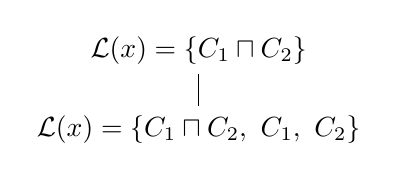
\begin{tikzpicture}[every text node part/.style={align=center},level 1/.style={level distance=1cm, sibling distance=3cm}]
\node [sibling distance=12cm] {$\mathcal{L}(x)=\{C_1\sqcap C_2\}$}
child { node []{$\mathcal{L}(x)=\{C_1\sqcap C_2,~C_1,~C_2\}$}
};
\end{tikzpicture} 
\end{center}
\item[$\sqcup$-rule:] if $C_1\sqcup C_2\in \mathcal{L}(x)$, $x$ is not indirectly blocked and $\{C_1,C_2\} \cap \mathcal{L}(x)\neq \emptyset$, then $ \mathcal{L}(x)\rightarrow 
\mathcal{L}(x)\cup \{C\}~for ~some ~C\in\{C_1,C_2\}$.
\begin{center}
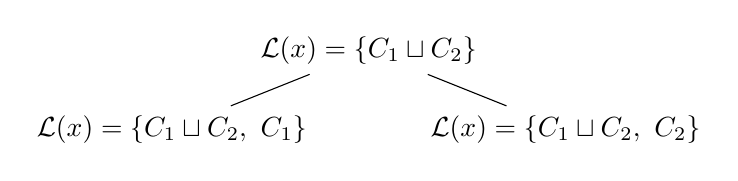
\begin{tikzpicture}[every text node part/.style={align=center},level 1/.style={level distance=1cm, sibling distance=5cm}]
\node [sibling distance=18cm] {$\mathcal{L}(x)=\{C_1\sqcup C_2\}$}
	      child{ node {$\mathcal{L}(x)=\{C_1\sqcup C_2,~C_1\}$}}
	      child{ node {$\mathcal{L}(x)=\{C_1\sqcup C_2,~C_2\}$}};
\end{tikzpicture} 
\end{center}
\item[$\exists$-rule:]  if $\exists r.C\in \mathcal{L}(x)$, $x$ is not blocked and $x$ has no $r$-neighbor $y$ with $C\notin \mathcal{L}(y)$, then create a new node $y$ 
with $\mathcal{E}(\langle x,y\rangle)$ and $\mathcal{L}(y)=\{C\}$.
\begin{center}
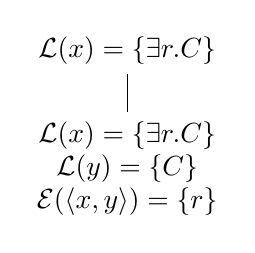
\begin{tikzpicture}[every text node part/.style={align=center},level 1/.style={level distance=1.5cm, sibling distance=3cm}]
\node [sibling distance=12cm] {$\mathcal{L}(x)=\{\exists r.C\}$}
child { node []{$\mathcal{L}(x)=\{\exists r.C\}$ \\ $\mathcal{L}(y)=\{C\}$ \\ $\mathcal{E}(\langle x,y \rangle)=\{r\}$}
};
\end{tikzpicture} 
\end{center}
% \textit{A short discussion:}
% \textit{In the $\exists$-rule, if $\exists r.C\in \mathcal{L}(x)$, a new node is added in two cases : \begin{inparaenum} \item when there exists an edge labeled with $\{r\}$ from $x$ to $y$ and 
% $C \notin  \mathcal{L}(y)$. \item when there does not exist an edge labeled with $\{r\}$ from $x$ to any other nodes. \end{inparaenum}}

\item[$\forall$-rule:] if $\forall r.C\in \mathcal{L}(x)$, $x$ is not indirectly blocked and there exists an $r$-neighbor $y$ of $x$ with $C\notin \mathcal{L}(y)$, then $ \mathcal{L}(y)\rightarrow  \mathcal{L}(y)\cup \{C\}$.
\begin{center}
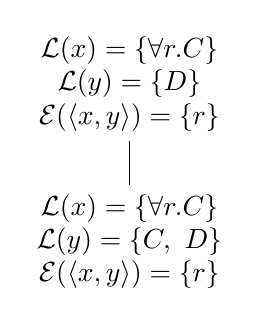
\begin{tikzpicture}[every text node part/.style={align=center},level 1/.style={level distance=2cm, sibling distance=3cm}]
\node [sibling distance=12cm] {$\mathcal{L}(x)=\{\forall r.C\}$\\ $\mathcal{L}(y)=\{D\}$ \\ $\mathcal{E}(\langle x,y \rangle)=\{r\}$}
child { node []{$\mathcal{L}(x)=\{\forall r.C\}$ \\ $\mathcal{L}(y)=\{C, ~D\}$ \\ $\mathcal{E}(\langle x,y \rangle)=\{r\}$}
};
\end{tikzpicture} 
\end{center}
\end{itemize}


The tableau is said to be complete  when there exists a clash in some node $x$ or none of the rules mentioned above can be applied in the tableau. 
For a given concept $D$, $D ~ is ~ satisfiable$ if the tableau is complete without a clash, otherwise   $D ~ is ~ unsatisfiable$.

\begin{mydef}(Clash)
A tableau contains a clash if, for a node $x$ and a concept $C$, $\{C,\neg C\}\subseteq \mathcal{L}(x)$.
\end{mydef}
\begin{center}
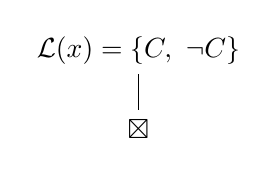
\begin{tikzpicture}[every text node part/.style={align=center},level 1/.style={level distance=1cm, sibling distance=3cm}]
\node [sibling distance=12cm] {$\mathcal{L}(x)=\{C,~\neg C \}$}
child { node []{$\boxtimes$}
};
\end{tikzpicture} 
\end{center}


\section{Qualitative spatial reasoning}\label{sec:qsr}
Qualitative spatial relations such as ``contains", ``left of", ``close to", ``between" can be categorized into three types: topological relations \cite{kuipers1978modeling}, 
directional relative relations and distances \cite{freeman1975modelling}. 
These relations are frequently used at a linguistic level by humans when describing a scene \cite{freksa1991qualitative}.
Even though quantitative information is more precise, human cannot use it as accurately as a machine.
Hence to qualitative representations to describe relations between spatial objects are crucial.
The aim of our study is to apply human knowledge to the description of qualitative relationships and the reasoning tasks with spatial objects in a complex scene.
Qualitative spatial reasoning deals with the following questions, among others:
 \begin{itemize}
  \item Can we recognize an object from known objects and their spatial relations?
  \item Which relationships are satisfied between two objects when their relationships are not explicitly described in a given  knowledge base?
  \item Is a recognized spatial arrangement of a scene consistent with the given knowledge of the scene?
 \end{itemize}
 
 The reasoning task can be summarized as follows:
 \begin{enumerate}
  \item Determining whether an object satisfies a spatial configuration, where an object is described by an observation of spatial arrangement and 
  a spatial configuration is defined using expert knowledge. Then the task is considered as a consistency checking  of the observed object with respect to the spatial configuration in 
  the knowledge base.
  \item Determining the relationship between two objects from other spatial arrangements. The implicit relations between two objects can be inferred by other known spatial relations
  in a spatial arrangement.
  \item Determining the consistency of a spatial arrangement in a given configuration of the scene with respect to a specific domain knowledge. This task verifies the consistency
  between the observation and the spatial configuration defined using expert knowledge.
 \end{enumerate}

 In this section, we discuss different representations of spatial relations and illustrate our formalism to perform spatial reasoning.

\subsection{State of the art}
Spatial relationship is an important factor for image interpretation in brain images due to the similar appearance among brain structures~\cite{Bloch2005fuzzy}.
Chen \textit{et al.} discussed a broad range of spatial relation representations~\cite{chen2013survey}. Different spatial calculi are summarized for various aspects of space 
(topology, direction, distance, object shape, etc.). Basic qualitative spatial relations are summarized in Table~\ref{tab:sr}.
\begin{center}
\begin{table}[h]
   \begin{tabular}{| l | c | c |}
    \hline
    Topological relations~\cite{randell1992spatial} & Directional relations & Distance relations \\ \hline
    dc (``disconnected from'') & left of & far from \\ 
    eq (``equal with'', ``identical'') & right of & close to \\
    po (``intersect with'', ``partially overlaps'') & above  &   \\
    ec (``external connected with'',``touches'', ``adjacent'') & below &  \\
    tpp (``tangential proper part of'') & in front of &  \\
    tppi (``inversion of tpp'') &  behind  &   \\
    ntpp (``not tangential proper part of'') &   &  \\
    ntppi (``inversion of ntpp'') &  &  \\
    \hline
  \end{tabular}
  \caption{Basic spatial relations.}
  \label{tab:sr}  
\end{table}
\end{center}
\subsubsection{Topology}
Topology has been mostly investigated in qualitative spatial representation and the most popular representation is based on \textit{Region Connection Calculus} (RCC)~\cite{cohn1997qualitative}.
The collection $\{dc,~eq,~po,~ec,~tpp,~tppi,~ntpp,~ntppi\}$ is a set of disjoint exhaustive topological relations defined as RCC8~\cite{randell1992spatial}.
Between any two objects in topological space, only one of eight relations can hold.
Therefore, a useful reasoning mechanism of RCC8 based on a composition table is proposed in~\cite{egenhofer1991reasoning} (Table~\ref{tab:comptable}).
Let $A,B,C$ be three objects in a topological space, both $A,B$ and $B,C$ are adjacent ($ec$). Then the possible relations between $A,C$ can be found within the table.
This reasoning mechanism allows answering the second and third questions of qualitative spatial reasoning problems. 
However, the composition table only gives possible relations and many of composition rules give no information like $dc(A,B)$ and $dc(B,C)$ (all the relations possibly
hold between $A$ and $C$ from the composition table).
Further, the RCC8 representation and composition table were constructed for determining a satisfaction problem 
in a specific arrangement~\cite{wessel2000obstacle,wessel00alcra}.
Unfortunately, the inference within this kind of representation is undecidable~\cite{wessel2000obstacle}. 
Afterwards, Lutz \textit{et al.} exploited qualitative reasoning in concrete domains with constraint satisfaction problems~\cite{lutz2007tableau}.
In the context of brain anatomy, only the inclusion relations are included in the work in~\cite{santos2012region}.
The property of transitivity  is emphasized in this context. 
 \begin{center}
 \begin{table}[H]
 %p{1cm} || p{1cm} | p{1cm} | p{1cm} | p{1cm} | p{1cm} |p{1cm} |p{1cm}| p{1cm}|
    \begin{tabular}{|p{1cm} || p{1.5cm} | p{1.5cm} | p{1.5cm} | p{1.5cm} | p{1.5cm} |p{1.5cm} |p{1.5cm}| p{1.5cm}| }
    \hline
      & $dc$ (B,C) & $\textbf{ec}$ $\textbf{(B,C)}$ & $eq$ (B,C) & $ntpp$  (B,C) & $tpp$ (B,C) &  $ntppi$ (B,C) & $tppi$ (B,C)& $op$ (B,C)\\ \hhline{|=|=|=|=|=|=|=|=|=|}
    $dc$ (A,B) & $dc$ or $ec$ or $eq$ or $ntpp$ or $tpp$ or $ntppi$ or $tppi$ or $op$  & $dc$ or $ec$ or $ntpp$ or $tpp$ or $op$ & $dc$ & $dc$ or $ec$ or $ntpp$ or $tpp$ or $op$ 
		& $dc$ or $ec$ or $ntpp$ or $tpp$ or $op$ & $dc$ &  $dc$ & $dc$ or $ec$ or $ntpp$ or $tpp$ or $op$ \\ \hline 
    $\textbf{ec}$ $\textbf{(A,B)}$ & $dc$ or $ec$ or $eq$ or $ntpp$ or $tpp$ or $ntppi$ or $tppi$ or $op$  & $\textbf{dc~or ec}$ $\textbf{or ntpp}$ $\textbf{or tpp}$ $\textbf{or op}$ & $dc$ 
    & $dc$ or $ec$ or $ntpp$ or $tpp$ or $op$ 	& $dc$ or $ec$ or $ntpp$ or $tpp$ or $op$ & $dc$ &  $dc$ & $dc$ or $ec$ or $ntpp$ or $tpp$ or $op$ \\ \hline 
    $eq$  (A,B) & $dc$ & $ec$ & $eq$ & $ntpp$ & $tpp$ & $ntppi$ & $tppi$ & $op$\\ \hline
    $ntpp$  (A,B)& $dc$ & $dc$ & $ntpp$ & $ntpp$ & $ntpp$ & $dc$ or $ec$ or $eq$ or $ntpp$ or $tpp$ or $ntppi$ or $tppi$ or $op$  & 
		  $dc$ or $ec$ or  $ntpp$ or $tpp$ or $op$& $dc$ or $ec$ or  $ntpp$ or $tpp$ or $op$\\ \hline
    $tpp$  (A,B)& $dc$ & $dc$ or $ec$  & $tpp$ & $ntpp$ & $tpp$ or $ntpp$ & $dc$ or $ec$ or $ntppi$ or $tppi$ or $op$ & $dc$ or $ec$ or $eq$ or $tpp$ or $tppi$ or $op$ &
		   $dc$ or $ec$ or $ntpp$ or $tpp$ or $op$ \\ \hline
    $ntppi$ (A,B)& $dc$ or $ec$ or $ntppi$ or $tppi$ or $op$ & $ntppi$ or $tppi$ or $op$  & $ntppi$ & $eq$ or $ntpp$ or $tpp$ or $tppi$ or $ntppi$ or $op$ &$tppi$ or $ntppi$ or $op$
		  & $ntppi$ &$ntppi$ & $tppi$ or $ntppi$ or $op$ \\ \hline
    $tppi$ (A,B)& $dc$ or $ec$ or $ntppi$ or $tppi$ or $op$  & $ec$ or $ntppi$ or $tppi$ or $op$ & $tppi$ & $ntpp$ or $tpp$ or $op$ & $eq$ or $tpp$ or $tppi$ or $op$ & $ntppi$  &
		  $ntppi$ or $tppi$ & $ntppi$ or $tppi$ or $op$\\ \hline
    $op$ (A,B)& $dc$ or $ec$ or $ntppi$ or $tppi$ or $op$ & $dc$ or $ec$ or $ntppi$ or $tppi$ or $op$ & $op$ & $ntpp$ or $tpp$ or $op$ & $ntpp$ or $tpp$ or $op$ &
		  $dc$ or $ec$ or $ntppi$ or $tppi$ or $op$  & $dc$ or $ec$ or $ntppi$ or $tppi$ or $op$ & $dc$ or $ec$ or $eq$ or $ntpp$ or $tpp$ or $ntppi$ or $tppi$ or $op$\\ \hline
    \end{tabular}
    \caption{The 64 compositions of binary topological relations between objects $A$ and $C$ via the third object $B$. Extracted from~\cite{egenhofer1991reasoning}.}
    \label{tab:comptable}
\end{table}
\end{center} 
\subsubsection{Direction}
Directional relations are seen as primarily important spatial relationships in brain anatomical images~\cite{Bloch2005fuzzy,fouquier2012sequential,Hudelot2008fuzzy,nempont2013constraint}.
As mentioned in~\cite{Bloch2005fuzzy}, a direction is defined by a \textit{target object}, a \textit{reference object} and a \textit{reference system}.
In an 3D space, directional relations are represented by six basic terms (e.g.: right, above, behind, etc.).
In order to compute directional relationships between two objects, many methods such as histograms of angles and morphological approaches are summarized in~\cite{Bloch2005fuzzy}.
Fuzzy representation is employed in these approaches. 
For instance, a fuzzy set (fuzzy landscape) representing the region of space where a given directional relation with a reference object is satisfied 
can be computed using morphological dilatation of the reference object.
The satisfaction degree of the direction between the target object and the reference object is evaluated by comparison between the target object and the fuzzy landscape.
In crisp logic, many researches are based on two categories: point based and extend object based (bounding box)~\cite{chen2013survey}.
However, both of two representation ignore the influence of objects forms. The representation is not as accurate to human intuition as fuzzy representation.
% Counter the intuition result by ignoring object form/shape.
% 
% based on mathematical morphology and fuzzy set.
% 
% \cite{santos2012region,cohn1997qualitative,Hudelot2008fuzzy,hudelot2008spatial,
% wessel2000obstacle,wessel00alcra,egenhofer1991reasoning,moratz2003qualitative}
% \subsubsection{Distance}

\subsection{Qualitative spatial reasoning in $\mathcal{ALCHI_{R^+}}$}
In this section, we give the logical formalism to represent qualitative spatial relationships as roles and  corresponding properties in terms of role axioms within a role box.
% As spatial relations are represented  by roles, a set of role axioms is exploited to model spatial relations.
% In Scenario 1, only topological relations are considered for the spatial reasoning task. 
% A collection (defined as RCC-8: $\{dc, ~eq,~po,~ec,~tpp,~tppi,~ntpp,~ntppi\}$)  is used as a set of disjoint exhaustive topological relations \cite{cohn1997qualitative}.
% In Scenarios 2 and 3, directional relations and distance relations are considered.
% A set of basic spatial relations used in our framework is represented in Table~\ref{tab:sr}. 
% In the following, we denote roles by $u,v,r$, possibly with subscripts. The basic syntax and semantics are described, then role axioms are introduced for spatial reasoning.

\subsubsection{Syntax and semantics of roles}
\begin{mydef}(Role syntax)
 Let $N_R$ be  a set of role names, the inverse roles and the negation of roles are represented by $r^-$ and $\neg r$.
 Complex roles are characterized with $r_1\sqcap r_2$ and $r_1\sqcup r_2$.
 Role axioms are used for modeling properties of roles such as inclusion ($r_1\sqsubseteq r_2$) and role composition ($r_1 \circ r_2$).
\end{mydef}
Table \ref{tab:synrole} describes a main syntax and semantics of roles for Description Logics.
\begin{center}
\begin{table}[h]
   \begin{tabular}{| l | c | r |}
    \hline
    Constructor & Syntax & Semantics \\ \hline
    Atomic role & $r$ & $r^\mathcal{I}\subseteq \Delta^\mathcal{I} \times \Delta^\mathcal{I}$ \\
    Inverse role & $r^-$ & $\{\langle x,y\rangle,~x\in \Delta^\mathcal{I},~y\in \Delta^\mathcal{I} | ~\langle y,x \rangle\in r^\mathcal{I}\}$ \\ 
    Role negation & $\neg r$ & $\Delta^\mathcal{I} \times \Delta^\mathcal{I} \setminus r^\mathcal{I}$ \\
    Role composition & $r_1\circ r_2$ & $\{\langle x,z\rangle, x\in \Delta^\mathcal{I},~z\in \Delta^\mathcal{I}| \exists y\in \Delta^\mathcal{I}, 
\langle x,y\rangle\in r_1^\mathcal{I}~and~\langle y,z\rangle\in r_2^\mathcal{I}\}$  \\
    Role conjunction & $r_1\sqcap r_2$ & $r_1^\mathcal{I} \cap r_2^\mathcal{I}$ \\
    Role disjunction & $r_1\sqcup r_2$ & $r_1^\mathcal{I} \cup r_2^\mathcal{I}$ \\
    Role inclusion & $r_1\sqsubseteq r_2$ &  $r_1^\mathcal{I} \subseteq r_2^\mathcal{I}$\\
    Role equivalence & $r_1\equiv r_2$ & $r_1^\mathcal{I} = r_2^\mathcal{I}$\\
    \hline
  \end{tabular}
  \caption{Basic relations}
  \label{tab:synrole}  
\end{table}
\end{center}

\begin{mydef}(Role inclusion axiom) 
 A role inclusion axiom is defined in the form:
 $$r\sqsubseteq s,$$
 where $r$ and $s$ are basic roles in $N_R$ or complex roles built with role constructors. A role equivalence $r\equiv s$ can be rewritten in the form $r\sqsubseteq s$ and $s\sqsubseteq r$.
\end{mydef}
\begin{mydef}(RBox)
A role box, denoted by RBox, is a finite set
% \footnote{ Jamal has noted ``$\mathfrak{C}$ is infinite''. But I do not understand very well. A RBox is independent of concept expressions, which
% represents a set of properties of roles.}
of axioms for $N_R$  based on a set of roles $\mathbf{R}=N_R\cup\{r^-| r\in N_R\}$, where $r^-$  represents the inversion of role $r$.
Based on role inclusion and role equivalence, role axioms characterize role properties as follows:
\begin{itemize}
 \item role composition: $u\circ v \sqsubseteq r_1\sqcup \cdots\sqcup r_n$ with $n\geqslant 1$, which is interpreted as 
 $(u\circ v)^\mathcal{I} \subseteq r_1^\mathcal{I} \cup \cdots \cup r_n^\mathcal{I}$. If there exist three interpretation elements $x,y,z\in \Delta^\mathcal{I}$, 
 $\langle x,y \rangle \in u^\mathcal{I}$ and $\langle y,z \rangle \in v^\mathcal{I}$ implies  $\langle x,z \rangle \in r_1^\mathcal{I} \cup \cdots \cup r_n^\mathcal{I}$. 
 \item transitive role: $r\circ r \sqsubseteq r$, which is interpreted as $(r\circ r)^\mathcal{I} \subseteq r^\mathcal{I}$. If there exist three interpretation elements
 $x,y,z\in \Delta^\mathcal{I}$, $\langle x,y \rangle \in r^\mathcal{I}$ and $\langle y,z \rangle \in r^\mathcal{I}$ implies  $\langle x,z \rangle \in r^\mathcal{I}$.
 \item inverse roles: $u \equiv v^-$, which is interpreted as $u^\mathcal{I} = v^{-\mathcal{I}}$. If there exist two interpretation elements  $x,y\in \Delta^\mathcal{I}$,
 then $\langle x,y \rangle \in u^\mathcal{I}$ iff $\langle y,x \rangle \in v^\mathcal{I}$.
 \item symmetric role: $r \equiv r^-$, which is interpreted as $r^\mathcal{I} = r^{-\mathcal{I}}$. If there exist two interpretation elements  $x,y\in \Delta^\mathcal{I}$,
 then $\langle x,y \rangle \in r^\mathcal{I}$ iff $\langle y,x \rangle \in r^\mathcal{I}$.
 \item disjoint roles: $u\sqsubseteq \neg v$. which is interpreted as $u^\mathcal{I} \subseteq \Delta^\mathcal{I} \setminus v^\mathcal{I}$ or $u^\mathcal{I}\cap v^\mathcal{I}=\emptyset$. 
 If there exist two interpretation elements  $x,y\in \Delta^\mathcal{I}$, 
$\langle x,y \rangle \in u^\mathcal{I}$ implies $\langle x,y \rangle \notin v^\mathcal{I}$.
\end{itemize}
\end{mydef}
The knowledge base used for spatial reasoning in our framework is built with three blocks: terminologies (TBox), role axioms (RBox) and assertions (ABox)
($\mathcal{K}=\{\mathcal{T},\mathcal{R},\mathcal{A}\}$).

To ensure the termination of tableau construction, a mechanism for detecting cyclic expansions called \textit{blocking} is used.
To define \textit{blocking}, we first introduce the term \textit{$r$-neighbor}.
\begin{mydef}($r$-neighbor)
In the tableau, an edge $\langle x,y \rangle$ labeled with role $r$ relates two nodes $x$ and $y$,
$y$ is called a successor of $x$ and $x$ is called  a predecessor of $y$. An ancestor is the transitive closure of predecessor,
where the transitive closure refers to an indirect reachability relation constructed from a set of direct edges.
A node $y$ is a $r$-neighbor of a node $x$ if
\begin{itemize}
\item $x$ is a predecessor of $y$ and $\mathcal{E}(\langle x,y\rangle)=\{r\}$.
% \item $y$ is a predecessor of $x$ and $\mathcal{E}(\langle y,x\rangle)=r^-$.
\end{itemize}
\end{mydef}


\begin{mydef}(Blocking)

\begin{itemize}
\item A node $x$ is directly blocked, which indicates that it has a unique ancestor $y$ such that $\mathcal{L}(y)=\mathcal{L}(x)$.
\item  Otherwise, it is indirectly blocked if its predecessor $y$ is blocked by another ancestor $u$.
\end{itemize}
A node $x$ is blocked if for some ancestor $y$, $y$ is blocked or $\mathcal{L}(y)=\mathcal{L}(x)$. 
\end{mydef}

\subsection{From image to symbolic representation}
The transformation of representation from low-level numerical data to symbolic level is first phase of the framework.
Concretely, objects and contextual information are extracted and represented within terminologies using an ABox.

In Figure \ref{fig:sub_flowchart}, the flowchart shows the general algorithm for qualitative spatial reasoning to implement. 
The focus of this reasoning service is the concept subsumption checking between a given hypothesis and the observation concept extracted from an image.
The hypothesis is a more specific description of the observation in the image interpretation task if it is subsumed by the observation.
The input of the algorithm is a segmented brain image. 
Using TIVOLI\footnote{\url{https://trac.telecom-paristech.fr/trac/project/tivoli/wiki}}
image processing toolbox, the context information is extracted (quantification values).
The quantification values of the spatial relationships are then transformed to qualitative spatial relations by a threshold. 
This observation is then transformed into a structural representation for the purpose of concept subsumption checking. 
To complete the concept subsumption checking, three elements are essential:
\begin{inparaenum}
 \item the hypothesis which is constructed manually for expected test;
 \item a knowledge base for expert knowledge representation;
 \item an inference process is formalized for the reasoning service. We exploit tableaux methods in this context.
\end{inparaenum}

The algorithm can be divided into two parts. The first part involves evaluating qualitative spatial relationships between segmented objects.
Segmented objects and their quantitative spatial relationships are then transformed manually as an ABox in the Description Logic formalism\footnote{I think the ABox can be built automatically
from the observation of image. However, the concept subsumption test depends on the constructed concept. This concept should be carefully selected from the ABox to get a desired result.}.
The second part contains the reasoning process guided by a knowledge base in a predefined logic formalism. The reasoning process is modeled as concept subsumption checking.
The hypothesis is considered as a more specific description of the observation if the decision process returns yes, otherwise the hypothesis does not belong to the subconcept of the observed concept.

The following sections will explain the details of each module.


The first part deals with the computation of qualitative relationships in a segmented image. 
In this module, TIVOLI image processing toolbox is used for extracting quantitative spatial relations between every two structures.
In a segmented 3D volumetric image $\mathbf{I}$, different structures in the image are labeled.
% with different gray level by a defined convention
For each pair of structures, the directional relations are calculated with the function t\_fuzzyRelativePosition for six main directions: left, right, above, below, in front of, behind.
Each direction is associated with a satisfaction degree.
The distances are evaluated with the function t\_distance and t\_mask. Minimum distance, mean distance and Hausdorff distance are all evaluated. 
% From the observation of test, we find out that ... (to be completed).

Computation process:
\begin{itemize}
 \item Initialization: the input of the process is a segmented image, with a known label for each structure of interest.
 \item Computation: for each pair of structures $a$ and $b$, we evaluate metric relations (directional relations and distances) of $a$ taking $b$ as the reference object 
 as well as the directional relations of  $b$ taking $a$ as the reference object. 
 \item The directional spatial relations are evaluated using t\_histoAngle by measuring between points of the two objects of interest or 
 t\_fuzzyRelativePosition by comparing the fuzzy landscape with a certain angle from reference structure and the target structure.
 \item The distances are evaluated using t\_distance and t\_mask. The minimum distance, mean distance and Hausdorff distance can be measured from the landscape propagated from the reference structure.
\end{itemize}

\subsubsection{Computation of direction between a pair of structures}
% \begin{figure}
%   \centering
%   \includegraphics[scale=0.4]{figures/cana_2d_53.jpg}
%   \caption{One slice of a brain volume with a tumor.}  \label{fig:brain}
% \end{figure}

% \begin{figure}
%   \centering
%   \includegraphics[scale=0.4]{figures/cana_seg_binary_53.jpg}
%   \caption{One slice of a segmented brain volume with a tumor.}  \label{fig:segbrain}
% \end{figure}
Two approaches of computations have been tested to evaluate a pair of structures from an image.
One is calculation of histogram of angles, and  the other is the morphological method by pattern matching between the structure and  the fuzzy directional landscape of the reference structure.
We take the left caudate nucleus (target object) and the left lateral ventricle (reference object) as an example to illustrate the computation\footnote{Here we use ``left'' to represent 
structures in the left part of image for the simplicity of visualization (i.e. the structure in the left part of image is the right part in the brain.)}.
The structures are presented in Figure. \ref{fig:cdlvl}.
% \begin{figure}
%   \centering
%         \begin{subfigure}[b]{0.3\textwidth}
%                 \includegraphics[width=\textwidth]{figures/LVr_2d_53.jpg}
%                 \caption{The left lateral ventricle}
%                 \label{fig:lvl}
%         \end{subfigure}
%         ~ 
%         \begin{subfigure}[b]{0.3\textwidth}
%                 \includegraphics[width=\textwidth]{figures/CDr_2d_53.jpg}
%                 \caption{The left caudate nucleus}
%                 \label{fig:cdl}
%         \end{subfigure}
%         \caption{One slice of a 3D volume }\label{fig:cdlvl}
% \end{figure}

The histogram of angles includes the count of angles of each pair of pixels in the left caudate nucleus and the left lateral ventricle.
The histogram is normalized and contains 256 bins as in Figure \ref{fig:histogram_angle}.
\begin{figure}
  \centering
  \includegraphics[scale=0.4]{figures/LVr_CDr_histo_angle_53.pdf}
  \caption{The normalized histogram of angles between the left caudate nucleus and the left lateral ventricle.
  The value of x-axis ranges from 0 to 255 representing the angle between $-\pi$ to $\pi$.}  \label{fig:histogram_angle}
\end{figure}

\begin{table}[H]
\begin{center}
   \begin{tabular}{| c || c | c | c | c |}
     \hline
     & right & left & above & below\\ \hline
     center of gravity of compatibility & 0.14  & 0.63 & 0.57  &  0.51 \\
     \hline
   \end{tabular}
    \caption{ The global evaluation is taken from the center of gravity of compatibility of angle histogram and direction fuzzy set.}\label{tab:cp_lvr_cnr}
     \end{center}
    \end{table}
From the figure, we observe that three peaks (greater than 0.75) appear around 30, 75, 255, which means the left caudate nucleus is strongly above and to the left of the left lateral ventricle.
The satisfaction degree can be computed with the observed histogram and the fuzzy set of a certain direction.
The global evaluation of a certain direction is obtained after the computation of compatibility fuzzy sets with respect to fuzzy relations.
The evaluation is the center of gravity of the compatibility fuzzy set as shown in Table \ref{tab:cp_lvr_cnr}.
``Left'', ``above'' and ``below'' relations are considered as the main direction between the left caudate nucleus and the left lateral ventricle.

We then illustrate the morphological approach for the evaluation. In Figure \ref{fig:before_landscape}, a fuzzy landscape for the relation ``below'' is computed with the help of morphological dilation operator.
In Table \ref{tab:direction_lvr_cnr}, the necessity, possibility and average values are computed using the fuzzy pattern matching. The necessity and possibility give an interval information of belief.
We take the average evaluation for quantification by a threshold (0.5). Therefore, the left caudate nucleus is considered as on the ``left'', ``above'' and ``below'' the left lateral ventricle,
which corresponds to our intuition.
% \begin{figure}
%   \centering
%   \includegraphics[scale=0.4]{figures/LVr_53_before.jpg}
%   \caption{Fuzzy landscape corresponding to the ``below'' position of the left lateral ventricle (high gray level represents the high membership values).}  \label{fig:before_landscape}
% \end{figure}

\begin{table}[H]
\begin{center}
   \begin{tabular}{| l || c | c | c | }
     \hline
     & Necessity & Possibility & Average value\\ \hline
     right & 0.12 & 0.61 & 0.41 \\ \hline
     left & 1.00 & 1.00 & 1.00 \\ \hline
%       above & 0.000000 & 1.000000 & 0.610771 \\ \hline
%       below  & 0.066667 & 1.000000 & 0.452501 \\ \hline
     above & 0.76 & 1.00 & 0.89 \\ \hline
     below  & 0.00 & 1.00 & 0.98 \\
     \hline
   \end{tabular}
    \caption{ The evaluation of satisfaction degrees of directional relations in the form of necessity, possibility, average between two structures.}\label{tab:direction_lvr_cnr}
     \end{center}
    \end{table}

%  
% If the hypothesis holds under the detected facts.
% 
% Discussion of computational cost.

\subsubsection{Computation of distances between a pair of structures}
The distances between the left caudate nucleus and the left lateral ventricle are given in Table \ref{tab:distance_cdr_lvr}. This table shows that minimum distance and Hausdorff distance satisfy the
symmetric property while the mean distance  does not. When we choose the minimum distance for the quantification and a threshold great than 1, the pair of structures are ``close to'' each other.
\begin{table}[H]
\begin{center}
   \begin{tabular}{| l || c | c | c | c | }
     \hline
     & Minimum distance & Mean distance & Hausdorff distance\\ \hline
     Ref:CNl, Tar:LVl & 1 mm & 5 mm & 99 mm\\ \hline
     %max: 99
     Ref:LVl, Tar:CNl & 1 mm & 30 mm & 99 mm\\ \hline
     %max: 15
   \end{tabular}
    \caption{ Different distances  between a pair of structures.}\label{tab:distance_cdr_lvr}
     \end{center}
    \end{table}
    
% Initialization: Input of a segmented image, followed by a label map, each structure is assigned with a gray level. 
% For every two structures, a target structure and a reference structure, all the directional spatial relations are computed with a satisfaction degree.
% The distance are also evaluated. The minimum distance is the smallest distance of the target structure in the distance landscape of reference structure.
% The mean distance is the calculated from the histogram of the distance. The Hausdorff distance is the largest of one of maximum distance if we switch the 
% reference structure and target structure.
% \section{Knowledge base}
In the knowledge base, we focus on the anatomy of the brain represented with Description Logics.
The brain structure concepts, qualitative spatial relationships and individuals of an observation are modeled as the signature of the defined Description Logic.
The taxonomy of brain structures and spatial configuration among the brain structures are described by the TBox.
The TBox contains a set of axioms which describes the structural hierarchies and their relational structures.
For example, 
Hemisphere is \textit{a part of} brain ($Hemisphere \sqsubseteq \exists isPartOf. Brain$).
The left lateral ventricle (LVl) is \textit{to the left of} and \textit{close to} the left caudate nucleus (CNl) ($LVr \sqsubseteq \exists (leftOf \sqcap closeTo). CNl$). 
The properties of the qualitative spatial relationships are described by the RBox.
For example, \textit{on the right of} is an inverse role of \textit{on the left of} ($rightOf \equiv leftOf^-$), and 
\textit{is part of} is a transitive role ($isPartOf \circ isPartOf \sqsubseteq isPartOf$).

The complete knowledge base is given as follows:
\begin{align*}
 TBox=\{ Hemisphere &\sqsubseteq \exists isPartOf. Brain\\
	 BrainStructure &\sqsubseteq \exists isPartOf. Brain\\
	 BrainDisease &\sqsubseteq \exists isPartOf. Brain \sqcap \neg BrainStructure\\
	 Tumor  &\sqsubseteq BrainDisease\\
	 LVl &\sqsubseteq BrainStructure \sqcap \sqsubseteq \exists (rightOf \sqcap closeTo). CNl\\
	 LVr &\sqsubseteq BrainStructure \sqcap \sqsubseteq \exists (leftOf \sqcap closeTo). CNr\\
	 CNl &\sqsubseteq BrainStructure\\
	 CNr &\sqsubseteq BrainStructure\\
	 WMl &\sqsubseteq BrainStructure\\
	 WMr &\sqsubseteq BrainStructure\\
	 PUl &\sqsubseteq BrainStructure\\
	 PUr &\sqsubseteq BrainStructure\\
	 THl &\sqsubseteq BrainStructure\\
	 THr &\sqsubseteq BrainStructure\}
\end{align*}

\begin{align*}
 RBox=\{ rightOf &\equiv leftOf^-\\
         above &\equiv below^- \\
	 closeTo &\equiv closeTo^- \\
	 farFrom &\equiv farFrom^- \\
	 isPartOf \circ isPartOf &\sqsubseteq isPartOf \\
	 hasPart \circ hasPart &\sqsubseteq hasPart\}
\end{align*}

% The ABox is used for describing the observation in the image.
% The spatial configuration describes the relationships between different structures.
The ABox represents the observation of recognized structures and the relationships with others.
For example, a region is recognized as the left caudate nucleus (CNl), denoted by $a$.
The region of brain is denoted by $c$. An unknown region is segmented and their relationships are computed.  
Such an observation can be represented as\footnote{At first, I assume to use a threshold to convert quantification measures to qualitative representations. However, the threshold 
is hard to choose. If we use a fuzzy ABox, only the spatial relations are assigned with a satisfaction degree. However, I have not read the reference about reasoning service on fuzzy Description Logics yet.}:
\begin{align*}
 ABox=\{ a&: CNl \\
	 b&: unknown \\
	 c&: Brain \\
	 \langle a,b\rangle &: rightOf, closeTo \\
	 \langle b,c\rangle &: isPartOf\}
\end{align*}
% so that the TBox of the knowledge base is modeled for the arrangement of brain structures
% and qualitative spatial relations used for the knowledge representation.
% The domain knowledge is represented in terms of Description Logics
OWL is a family of ontology language based on Description Logics. 
We use OWL API to create the knowledge base which consists of the TBox, the RBox and the ABox.
The signature involves brain structures as atomic concepts and qualitative spatial relations as roles.
With OWL API, the TBox  and RBox can be represented with the class OWLAxiom.
% In RBox we define the corresponding properties of roles for qualitative spatial relations.
This kind of knowledge representation provides a description of a domain as well as the reasoning formalisms about the domain.




\subsection{Spatial reasoning using tableaux method}
\begin{mydef}[Interpretation]
An interpretation $\mathcal{I}=(\Delta^\mathcal{I},\cdot^\mathcal{I})$ provides the semantics of concepts and roles. $\Delta^\mathcal{I}$ is a non-empty set which indicates the entire
``world" of the application domain. $\cdot^\mathcal{I}$ is an interpretation function which connects concept and individual symbols to $\Delta^\mathcal{I}$ and roles to $\Delta^\mathcal{I} \times \Delta^\mathcal{I}$.
\begin{itemize}
 \item Every concept $C\in N_C$ is interpreted as a subset of $\Delta^\mathcal{I}$, represented by $C^\mathcal{I}\subseteq \Delta^\mathcal{I}$.
 \item Every  role $r$ is interpreted as a subset of $\Delta^\mathcal{I}\times\Delta^\mathcal{I}$, denoted as $r^\mathcal{I}\subseteq \Delta^\mathcal{I}\times\Delta^\mathcal{I}$.
 \item Every individual $a \in N_I$ is interpreted as an element in the set $\Delta^\mathcal{I}$, denoted as $a^\mathcal{I} \in \Delta^\mathcal{I}$.
\end{itemize}
\end{mydef}


The table of syntax and semantics of $\mathcal{ALCHI_{R_+}}$ is shown as follows:
 \begin{center}
 \begin{table}[H]
    \begin{tabular}{|p{4cm} | p{2cm} | p{10cm}| }
    \hline
      Name & Syntax & Semantics \\ \hline
    Top & $\top$ & $\Delta^\mathcal{I}$ \\
    Bottom & $\bot$ & $\emptyset$ \\ 
    Negation & $\neg C$ & $\Delta^\mathcal{I}\setminus C^\mathcal{I}$ \\ 
    Conjunction & $C\sqcap D$ & $C^\mathcal{I}\cap D^\mathcal{I}$  \\  
    Disjunction & $C\sqcup D$ &  $C^\mathcal{I}\cup D^\mathcal{I}$ \\  
    Existential restriction & $\exists r.C$ & $\{x\in \Delta^\mathcal{I}~|~ \exists y\in \Delta^\mathcal{I}, \langle x,y\rangle \in r^\mathcal{I}~and~y\in C^\mathcal{I}\}$ \\ 
    Universal restriction & $\forall r.C$ & $\{x\in \Delta^\mathcal{I}~|~ \forall~y\in \Delta^\mathcal{I}, \langle x,y\rangle \in r^\mathcal{I}~implies~y\in C^\mathcal{I}\}$ \\ \hline
    Atomic role & $r$ & $r^\mathcal{I}\subseteq \Delta^\mathcal{I} \times \Delta^\mathcal{I}$\\
    Inverse role & $r^-$ & $\{(x,y),~x\in \Delta^\mathcal{I},~y\in \Delta^\mathcal{I} | ~(y,x)\in r^\mathcal{I}\}$\\ 
    Role composition & $r_1\circ r_2$ & $\{(x,z), x\in \Delta^\mathcal{I},~z\in \Delta^\mathcal{I}| \exists y\in \Delta^\mathcal{I},(x,y)\in r_1^\mathcal{I}~and~(y,z)\in r_2^\mathcal{I}\}$\\
    Role conjunction & $r_1\sqcap r_2$ & $r_1^\mathcal{I} \cap r_2^\mathcal{I}$ \\
    Role disjunction & $r_1\sqcup r_2$ & $r_1^\mathcal{I} \cup r_2^\mathcal{I}$ \\
    Role inclusion & $r_1\sqsubseteq r_2$ &  $r_1^\mathcal{I} \subseteq r_2^\mathcal{I}$\\
    Role equivalence & $r_1\equiv r_2$ & $r_1^\mathcal{I} = r_2^\mathcal{I}$\\    \hline
    Subsumption & $C\sqsubseteq D$ & $C^\mathcal{I}\subseteq D^\mathcal{I}$ for all $\mathcal{I}$\\
    Concept Definition & $C\equiv D$ & $C^\mathcal{I}= D^\mathcal{I}$ for all $\mathcal{I}$\\ \hline
    Concept assertion & $a:C$ & $a^\mathcal{I}\in C^\mathcal{I}$ \\
    Role assertion & $(a,b):r$ & $(a^\mathcal{I},b^\mathcal{I})\in r^\mathcal{I}$ \\ \hline
    \end{tabular}
    \caption{Syntax and interpretations of $\mathcal{ALCHI_{R_+}}$.}
    \label{tab:interpretation}
\end{table}
\end{center} 
A tableaux method tries to check satisfiability of a concept $D$ by finding a model for $D$. The tableaux is constructed by applying a set of expansion rules. The model contains a set of 
interpretation elements and associated concepts for each interpretation element. These concepts are restricted to subsets of subconcepts of $D$ ($sub(D)$). The subconcept of a concept $D$ is defined as
follows:
\begin{mydef}[Subconcept~\cite{horrocks1999description}]
 A subconcept of a concept $D$ is the concept occurring in $D$. $sub(\cdot)$ is the set of all subconcepts:
 \begin{align*}
 sub(A)&=\{A\}~for~concept~names~A\in N_C\\
 sub(C\sqcap E)&=\{C\sqcap E\}\cup sub(C)\cup sub(E)\\
 sub(C\sqcup E)&=\{C\sqcup E\}\cup sub(C)\cup sub(E)\\
 sub(\exists r.C)&=\{\exists r.C\}\cup sub(C)\\
 sub(\forall r.C)&=\{\forall r.C\}\cup sub(C)
 \end{align*}

\end{mydef}



\begin{mydef}[$\mathcal{ALCHI_{R+}}$ tableaux~\cite{horrocks1999description}]
Let $D$ be an $\mathcal{ALCHI_{R+}}$ concept in negation normal form (NNF) and let $R_D$ be the set of roles in $\mathcal{ALCHI_{R+}}$, a tableau $T$ for $D$ is defined as a triple 
$(\mathbf{S},\mathcal{L}, \mathcal{E})$, where $\mathbf{S}$ is a set of interpretation elements; 
$\mathcal{L}$ relates each interpretation element to a set of concepts occurring in $D$ ($\mathcal{L}:\mathbf{S}\rightarrow\mathcal{P}(sub(D))$
\footnote{$\mathcal{P}(sub(D))$ is the power set of $sub(D)$.}); 
$\mathcal{E}$ relates each pair of interpretation elements to a set of roles in $R_D$  ($\mathcal{E}:\mathbf{S}\times\mathbf{S}\rightarrow \mathcal{P}(R_D)$). 

The decision procedure to check the satisfiability of a given concept $D$ is based on constructing a model using the tableau method. 
Let $x$ and $y$ be two interpretation elements in $\mathbf{S}$ ($x,~y\in \mathbf{S}$), $C,E$ be two concepts occurring in $D$ and $r\in R_D$.
The model is constructed as a tree structure where each node corresponds to an element of interpretation $x\in \Delta^\mathcal{I}$.
The node is labeled with a set of concepts $\mathcal{L}(x)$.
The edge between the nodes $x$ and $y$ is labeled with corresponding roles $r\in\mathcal{E}(\langle x,y \rangle)$.
The following conditions hold:
\begin{enumerate}
\item if $C\in \mathcal{L}(x)$, then $\neg C\notin\mathcal{L}(x)$.
\item if $C\sqcap E\in \mathcal{L}(x)$, then $ C\in\mathcal{L}(x)$ and $ E\in\mathcal{L}(x)$.
\item if $C\sqcup E\in \mathcal{L}(x)$, then $ C\in\mathcal{L}(x)$ or $ E\in\mathcal{L}(x)$.
\item if $\exists r.C\in \mathcal{L}(x)$, then there exists some $y\in \mathbf{S}$  such that $r \in \mathcal{E}(\langle x,y\rangle)$ and $C\in\mathcal{L}(y)$.
\item if $\forall r.C\in \mathcal{L}(x)$, then for all  $y \in \mathbf{S}$ such that $r \in \mathcal{E}(\langle x,y\rangle)$, $C\in\mathcal{L}(y)$.
\item if $\forall r.C\in \mathcal{L}(x)$, for all $y \in \mathbf{S}$ such that $r \in \mathcal{E}(\langle x,y\rangle)$ and $r$ is a transitive role
\footnote{When $r$ is a transitive role, a possible model can be imagined for $y$ (the successor of $x$ and $r\in\mathcal{E}(\langle x,y\rangle)$): 
$y$ has a successor $z$, where $r\in\mathcal{E}(\langle y,z\rangle)$. In the RBox, the transitive role is defined as $r\circ r\sqsubseteq r$. If $\forall r.C\in \mathcal{L}(x)$, then 
$\forall r\circ r.C\in \mathcal{L}(x)$. Therefore, for $x$ $r$-successor $y$, $\forall r.C\in \mathcal{L}(y)$.}, then $\forall r.C\in \mathcal{L}(y)$.
% \item if $\forall r.C\in \mathcal{L}(x)$, for all $y \in \mathbf{S}$ such that $v \in \mathcal{E}(\langle x,y\rangle)$, $v\sqsubseteq r$ (or $v^-\sqsubseteq r^-$) and $v$ is a transitive role, then $\forall v.C\in \mathcal{L}(y)$.
\item $r \in \mathcal{E}(\langle x,y\rangle)$ iff  $ r^-\in \mathcal{E}(\langle y,x\rangle)$.
\item if $ r\in \mathcal{E}(\langle x,y\rangle)$ and $r\sqsubseteq v$ (or $r^-\sqsubseteq v^-$) then  $v \in \mathcal{E}(\langle x,y\rangle)$.
\end{enumerate}

\end{mydef}
\subsection{Example}
 The complete knowledge base is given as follows:
\begin{align*}
 TBox=\{ Hemisphere &\sqsubseteq \exists isPartOf. Brain\\
	 BrainStructure &\sqsubseteq \exists isPartOf. Brain\\
	 BrainDisease &\sqsubseteq \exists isPartOf. Brain \sqcap \neg BrainStructure\\
	 Tumor  &\sqsubseteq BrainDisease\\
	 LVl &\sqsubseteq BrainStructure \sqcap \exists (rightOf \sqcap closeTo). CNl\\
	 LVr &\sqsubseteq BrainStructure \sqcap \exists (leftOf \sqcap closeTo). CNr\\
	 CNl &\sqsubseteq BrainStructure\\
	 CNr &\sqsubseteq BrainStructure\}
% 	 WMl &\sqsubseteq BrainStructure\\
% 	 WMr &\sqsubseteq BrainStructure\\
% 	 PUl &\sqsubseteq BrainStructure\\
% 	 PUr &\sqsubseteq BrainStructure\\
% 	 THl &\sqsubseteq BrainStructure\\
% 	 THr &\sqsubseteq BrainStructure\}
\end{align*}
The role axioms are described as:
\begin{align*}
 RBox=\{ rightOf &\equiv leftOf^-\\
         above &\equiv below^- \\
	 closeTo &\equiv closeTo^- \\
	 farFrom &\equiv farFrom^- \\
	 isPartOf \circ isPartOf &\sqsubseteq isPartOf \\
	 hasPart \circ hasPart &\sqsubseteq hasPart\\
	 isPartOf &\equiv hasPart^-\}
\end{align*}

% The ABox is used for describing the observation in the image.
% The spatial configuration describes the relationships between different structures.
The ABox represents the observation of structures in an image and the relationships between them.
In this example, both recognized and unrecognized structures are represented by individuals. Spatial relations between the unknown structure and
recognized structures are represented by roles.
For instance, a region is recognized as the left caudate nucleus (CNl), denoted by $a$.
The region of brain is denoted by $c$. An unknown region is segmented and their relationships are computed.  
Such an observation can be represented as
% \footnote{At first, I assume to use a threshold to convert quantification measures to qualitative representations. However, the threshold 
% is hard to choose. If we use a fuzzy ABox, only the spatial relations are assigned with a satisfaction degree. However, I have not read the reference about reasoning service on fuzzy Description Logics yet.}:
\begin{align*}
 ABox=\{ a&: CNl \\
	 b&: unknown \\
	 c&: Brain \\
	 \langle a,b\rangle &: leftOf, closeTo \\
	 \langle b,c\rangle &: isPartOf\}
\end{align*}

% In an image understanding application, we reason about a description which explains a given image in a certain domain.
In this example, the ABox describes an observation of a given scene and the objective is to find a reasonable description of  the unknown object $b$.
% This type of reasoning can be treated as an abductive reasoning.
A possible hypothesized description is $LVl\sqcap \exists isPartOf.Hemisphere$.
The hypothesis can be verified by a concept subsumption checking: $\mathcal{K} \vDash H\sqsubseteq O$, where $H$ is the explained concept for the observation $O$.
To check subsumption of two concepts $H$ and $O$, $\mathcal{K} \vDash H\sqcap \neg O \sqsubseteq \bot$ is required to prove that $H\sqcap \neg O$ is unsatisfiable.

In this example, $O\equiv \exists (leftOf^-\sqcap closeTo^-). CNl\sqcap \exists isPartOf.Brain$ and $H\equiv LVl\sqcap \exists isPartOf.Hemisphere$.
Let $x$ be the interpretation element of the concept $H\sqcap \neg O$. 

The tableau is initialized with $\mathcal{L}(x)=\{ LVl\sqcap \exists isPartOf.Hemisphere\sqcap \forall (leftOf^-\sqcap closeTo^-).\neg CNl\sqcup \forall isPartOf.\neg Brain\}$.
The $\sqcap$, $\sqcup$ rules are applied and we obtain:
\begin{center}
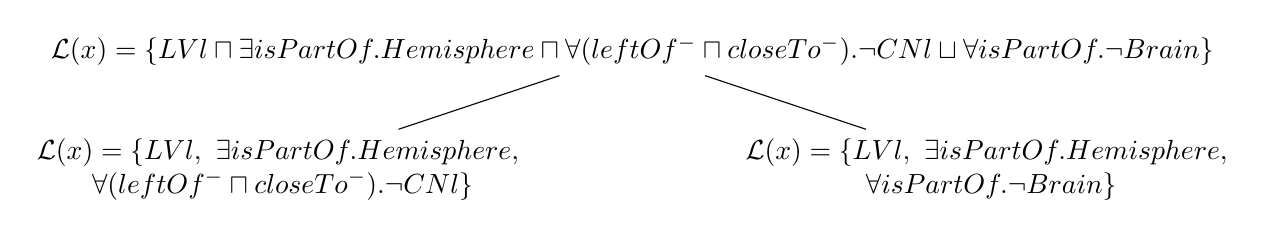
\begin{tikzpicture}[every text node part/.style={align=center},level 1/.style={level distance=1.5cm, sibling distance=9cm}]
\node [sibling distance=18cm] {$\mathcal{L}(x)=\{ LVl\sqcap \exists isPartOf.Hemisphere\sqcap \forall (leftOf^-\sqcap closeTo^-).\neg CNl\sqcup \forall isPartOf.\neg Brain\}$}
	      child{ node {$\mathcal{L}(x)=\{ LVl,~\exists isPartOf.Hemisphere,$\\$~\forall (leftOf^-\sqcap closeTo^-).\neg CNl\}$}}
	      child{ node {$\mathcal{L}(x)=\{ LVl,~\exists isPartOf.Hemisphere,$\\$~\forall isPartOf.\neg Brain\}$}};
\end{tikzpicture} 
\end{center}

To integrate terminological knowledge, axioms like $C\sqsubseteq D$ in the TBox can be internalized into single concepts ($\neg C\sqcup D$) and added to $\mathcal{L}(x)$. Here, for the sake of simplicity 
of demonstration, we only add the internalization of the axiom $LVl \sqsubseteq BrainStructure \sqcap  \exists (rightOf \sqcap closeTo). CNl$ for the first branch.
\begin{center}
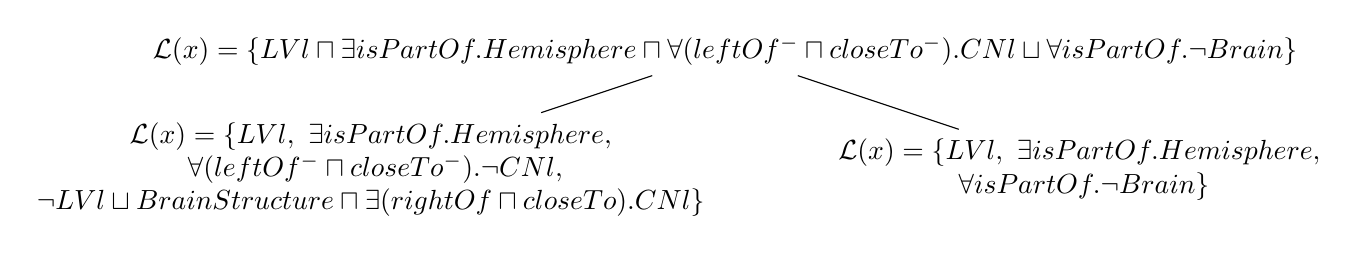
\begin{tikzpicture}[every text node part/.style={align=center},level 1/.style={level distance=1.5cm, sibling distance=9cm}]
\node [sibling distance=18cm] {$\mathcal{L}(x)=\{ LVl\sqcap \exists isPartOf.Hemisphere\sqcap \forall (leftOf^-\sqcap closeTo^-).CNl\sqcup \forall isPartOf.\neg Brain\}$}
	      child{ node {$\mathcal{L}(x)=\{ LVl,~\exists isPartOf.Hemisphere,$\\$~\forall (leftOf^-\sqcap closeTo^-).\neg CNl,$\\$\neg LVl \sqcup BrainStructure \sqcap \exists (rightOf \sqcap closeTo).CNl\}$}}
	      child{ node {$\mathcal{L}(x)=\{ LVl,~\exists isPartOf.Hemisphere,$\\$~\forall isPartOf.\neg Brain\}$}};
\end{tikzpicture}  
\end{center}

We then apply $\sqcup$ and $\sqcap$ rules again on the first branch:
\begin{center}
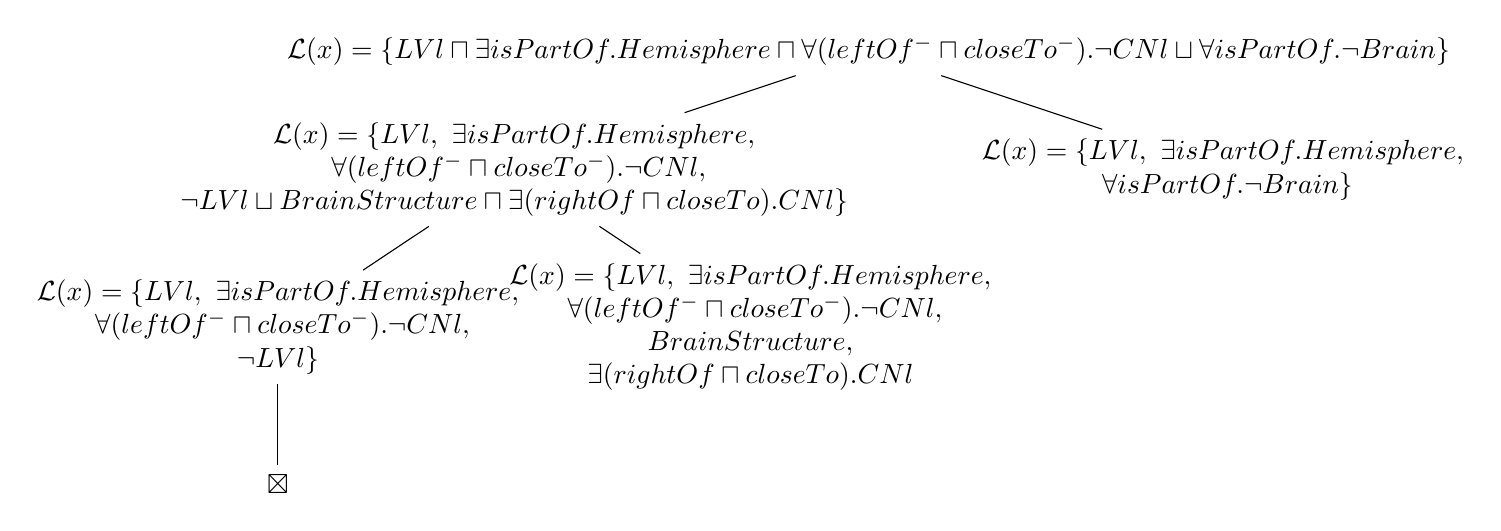
\begin{tikzpicture}[every text node part/.style={align=center},level 1/.style={level distance=1.5cm, sibling distance=9cm}, level 2/.style={level distance=2cm, sibling distance=6cm}]
\node [sibling distance=18cm] {$\mathcal{L}(x)=\{ LVl\sqcap \exists isPartOf.Hemisphere\sqcap \forall (leftOf^-\sqcap closeTo^-).\neg CNl\sqcup \forall isPartOf.\neg Brain\}$}
	      child{ node {$\mathcal{L}(x)=\{ LVl,~\exists isPartOf.Hemisphere,$\\$~\forall (leftOf^-\sqcap closeTo^-).\neg CNl,$\\$\neg LVl \sqcup BrainStructure \sqcap \exists (rightOf \sqcap closeTo).CNl\}$}
	      		    child{ node {$\mathcal{L}(x)=\{ LVl,~\exists isPartOf.Hemisphere,$\\$~\forall (leftOf^-\sqcap closeTo^-).\neg CNl,$\\$\neg LVl\}$}
				  child{ node{$\boxtimes$}}}
		            child{ node {$\mathcal{L}(x)=\{ LVl,~\exists isPartOf.Hemisphere,$\\$~\forall (leftOf^-\sqcap closeTo^-). \neg CNl,$\\$BrainStructure,$\\$\exists (rightOf \sqcap closeTo).CNl$}}}
	      child{ node {$\mathcal{L}(x)=\{ LVl,~\exists isPartOf.Hemisphere,$\\$~\forall isPartOf.\neg Brain\}$}};
\end{tikzpicture}  
\end{center}

A clash ($LVl,~\neg LVl$) is detected in the first part of the first branch (closed). We then apply $\exists$ on the second part:
\begin{center}
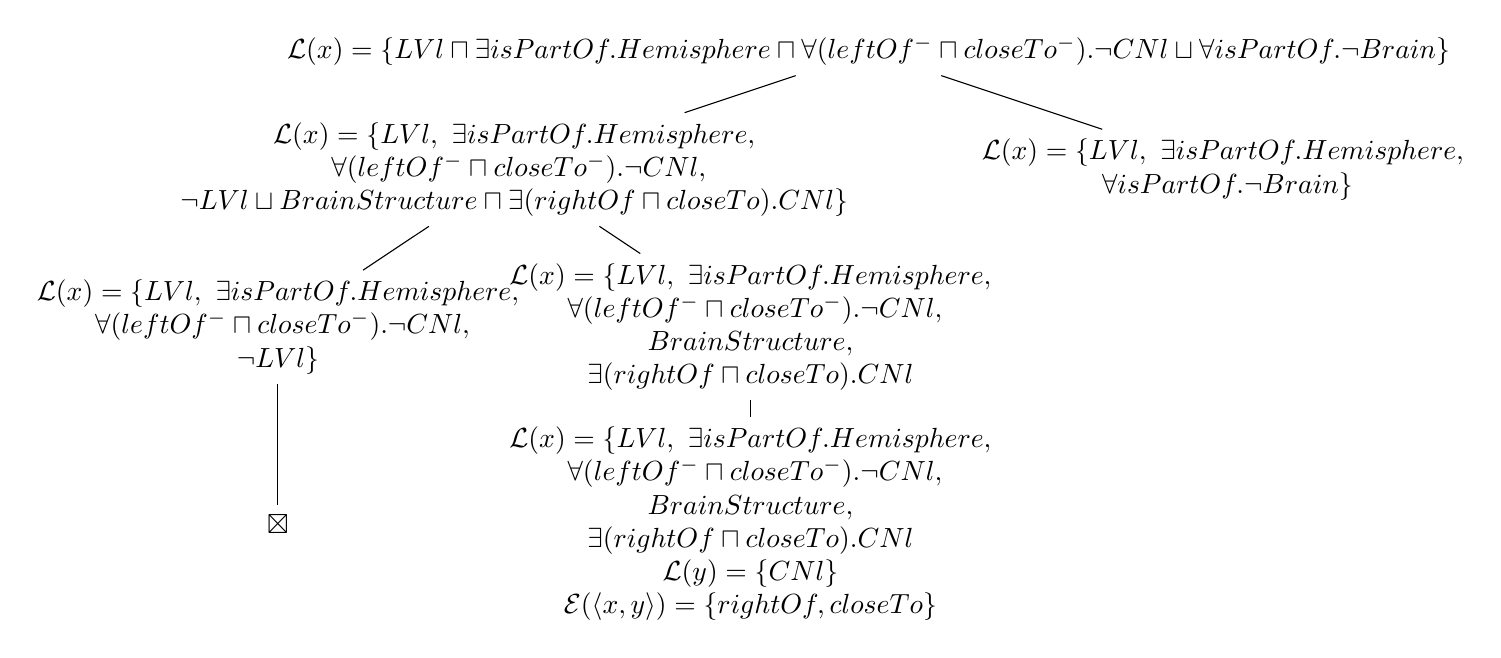
\begin{tikzpicture}[every text node part/.style={align=center},level 1/.style={level distance=1.5cm, sibling distance=9cm}, level 2/.style={level distance=2cm, sibling distance=6cm},
level 3/.style={level distance=2.5cm, sibling distance=6cm}]
\node [sibling distance=18cm] {$\mathcal{L}(x)=\{ LVl\sqcap \exists isPartOf.Hemisphere\sqcap \forall (leftOf^-\sqcap closeTo^-).\neg CNl\sqcup \forall isPartOf.\neg Brain\}$}
	      child{ node {$\mathcal{L}(x)=\{ LVl,~\exists isPartOf.Hemisphere,$\\$~\forall (leftOf^-\sqcap closeTo^-).\neg CNl,$\\$\neg LVl \sqcup BrainStructure \sqcap \exists (rightOf \sqcap closeTo).CNl\}$}
	      		    child{ node {$\mathcal{L}(x)=\{ LVl,~\exists isPartOf.Hemisphere,$\\$~\forall (leftOf^-\sqcap closeTo^-).\neg CNl,$\\$\neg LVl\}$}
				  child{ node{$\boxtimes$}}}
		            child{ node {$\mathcal{L}(x)=\{ LVl,~\exists isPartOf.Hemisphere,$\\$~\forall (leftOf^-\sqcap closeTo^-).\neg CNl,$\\$BrainStructure,$\\$\exists (rightOf \sqcap closeTo).CNl$}
				  child{ node {$\mathcal{L}(x)=\{ LVl,~\exists isPartOf.Hemisphere,$\\
				  $~\forall (leftOf^-\sqcap closeTo^-).\neg CNl,$\\$BrainStructure,$\\$\exists (rightOf \sqcap closeTo).CNl$\\
				  $\mathcal{L}(y)=\{CNl\}$\\
				  $\mathcal{E}(\langle x,y \rangle)=\{rightOf,closeTo\}$}}}}
	      child{ node {$\mathcal{L}(x)=\{ LVl,~\exists isPartOf.Hemisphere,$\\$~\forall isPartOf.\neg Brain\}$}};
\end{tikzpicture}  
\end{center}

Because of inverse role axiom in the RBox, we can add inverse roles in $\mathcal{E}(\langle x,y \rangle)$ and apply  $\forall$ rule on the second part:
\begin{center}
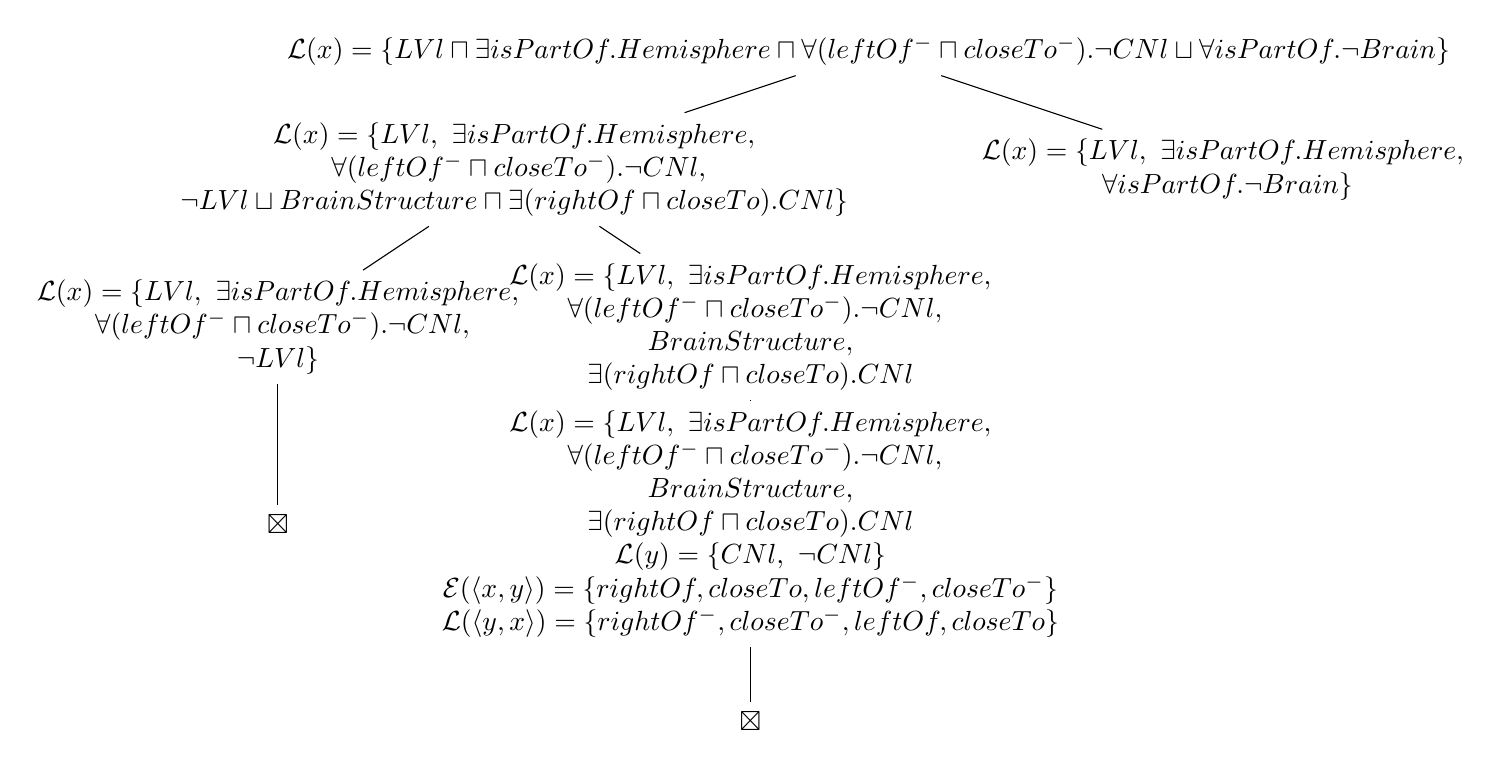
\begin{tikzpicture}[every text node part/.style={align=center},level 1/.style={level distance=1.5cm, sibling distance=9cm}, level 2/.style={level distance=2cm, sibling distance=6cm},
level 3/.style={level distance=2.5cm, sibling distance=6cm}]
\node [sibling distance=18cm] {$\mathcal{L}(x)=\{ LVl\sqcap \exists isPartOf.Hemisphere\sqcap \forall (leftOf^-\sqcap closeTo^-).\neg CNl\sqcup \forall isPartOf.\neg Brain\}$}
	      child{ node {$\mathcal{L}(x)=\{ LVl,~\exists isPartOf.Hemisphere,$\\$~\forall (leftOf^-\sqcap closeTo^-).\neg CNl,$\\$\neg LVl \sqcup BrainStructure \sqcap \exists (rightOf \sqcap closeTo).CNl\}$}
	      		    child{ node {$\mathcal{L}(x)=\{ LVl,~\exists isPartOf.Hemisphere,$\\$~\forall (leftOf^-\sqcap closeTo^-).\neg CNl,$\\$\neg LVl\}$}
				  child{ node{$\boxtimes$}}}
		            child{ node {$\mathcal{L}(x)=\{ LVl,~\exists isPartOf.Hemisphere,$\\$~\forall (leftOf^-\sqcap closeTo^-).\neg CNl,$\\$BrainStructure,$\\$\exists (rightOf \sqcap closeTo).CNl$}
				  child{ node {$\mathcal{L}(x)=\{ LVl,~\exists isPartOf.Hemisphere,$\\
				  $~\forall (leftOf^-\sqcap closeTo^-).\neg CNl,$\\$BrainStructure,$\\$\exists (rightOf \sqcap closeTo).CNl$\\
				  $\mathcal{L}(y)=\{CNl,~\neg CNl\}$\\
				  $\mathcal{E}(\langle x,y \rangle)=\{rightOf,closeTo,leftOf^-,closeTo^-\}$\\
				  $\mathcal{L}(\langle y,x\rangle)=\{rightOf^-,closeTo^-,leftOf,closeTo\}$}
				  child{ node{$\boxtimes$}}}}}
	      child{ node {$\mathcal{L}(x)=\{ LVl,~\exists isPartOf.Hemisphere,$\\$~\forall isPartOf.\neg Brain\}$}};
\end{tikzpicture}  
\end{center}

The first branch of the tableau is closed because of the clash of $CNl$ and $\neg CNl$ in the second part. We then explore the second branch. At first we apply the $\exists$ rule and then $\forall$ rule:
\begin{center}
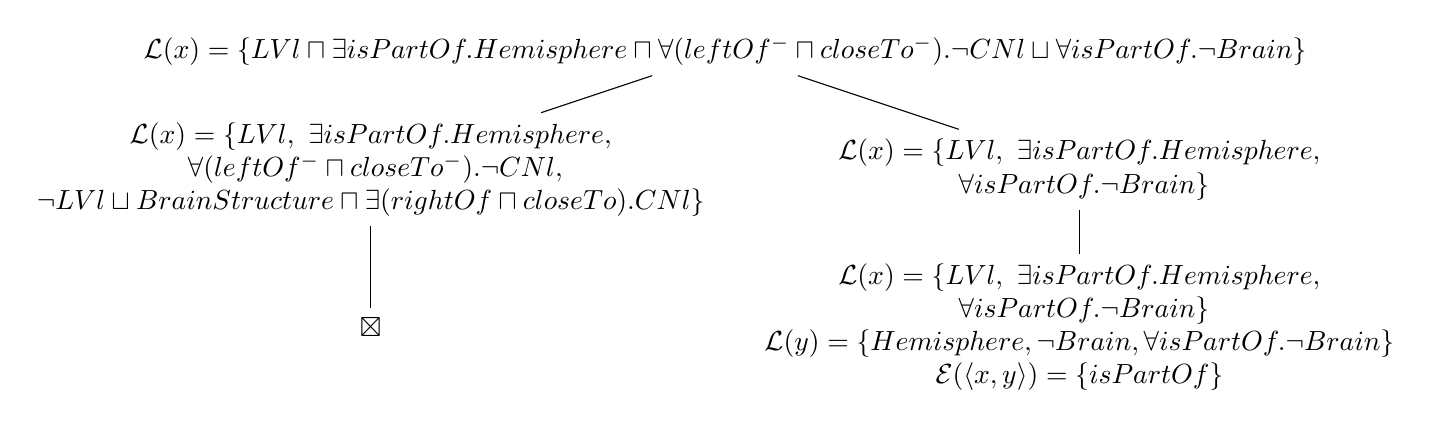
\begin{tikzpicture}[every text node part/.style={align=center},level 1/.style={level distance=1.5cm, sibling distance=9cm}, level 2/.style={level distance=2cm, sibling distance=6cm},
level 3/.style={level distance=2.5cm, sibling distance=6cm}]
\node [sibling distance=18cm] {$\mathcal{L}(x)=\{ LVl\sqcap \exists isPartOf.Hemisphere\sqcap \forall (leftOf^-\sqcap closeTo^-).\neg CNl\sqcup \forall isPartOf.\neg Brain\}$}
	      child{ node {$\mathcal{L}(x)=\{ LVl,~\exists isPartOf.Hemisphere,$\\$~\forall (leftOf^-\sqcap closeTo^-).\neg CNl,$\\$\neg LVl \sqcup BrainStructure \sqcap \exists (rightOf \sqcap closeTo).CNl\}$}
				  child{ node{$\boxtimes$}}}
	      child{ node {$\mathcal{L}(x)=\{ LVl,~\exists isPartOf.Hemisphere,$\\$~\forall isPartOf.\neg Brain\}$}
		     child{ node{$\mathcal{L}(x)=\{ LVl,~\exists isPartOf.Hemisphere,$\\$~\forall isPartOf.\neg Brain\}$\\
				  $\mathcal{L}(y)=\{ Hemisphere, \neg Brain, \forall isPartOf. \neg Brain\}$\\
				  $\mathcal{E}(\langle x,y \rangle)=\{isPartOf\}$}}};
\end{tikzpicture}  
\end{center}

The axiom $Hemisphere \sqsubseteq \exists isPartOf.Brain$ is internalized and added into $\mathcal{L}(y)$. Then we continue to extend the second branch with expansion rules:
\begin{center}
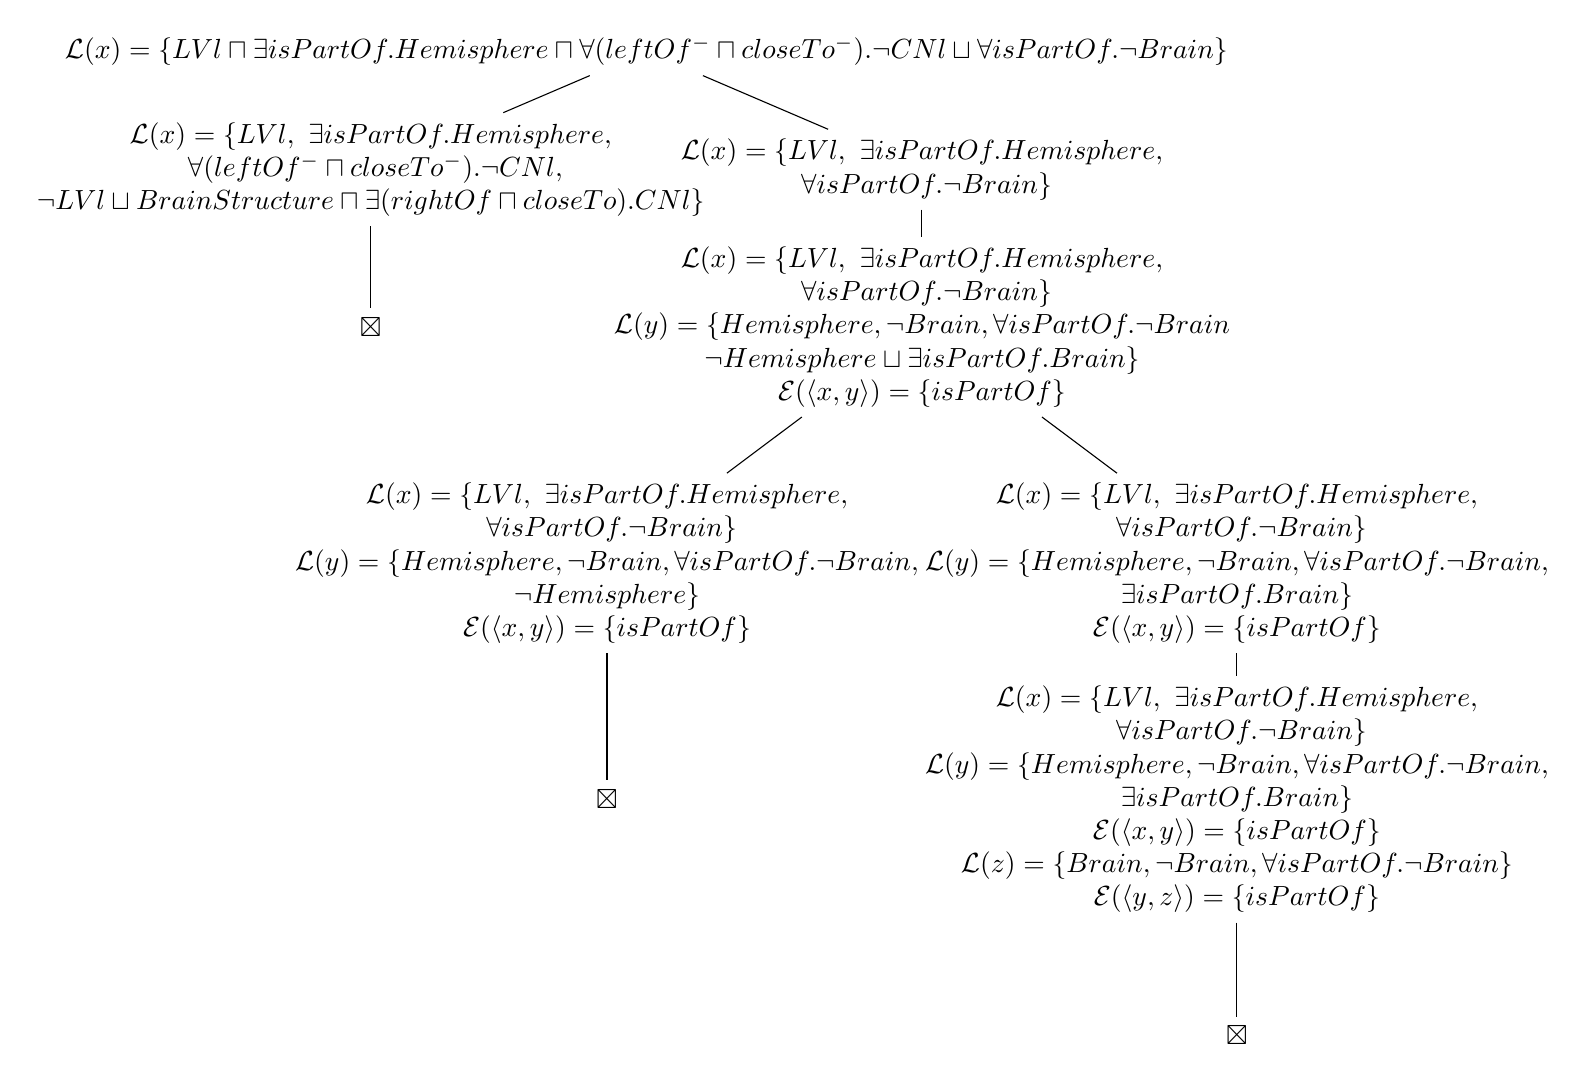
\begin{tikzpicture}[every text node part/.style={align=center},level 1/.style={level distance=1.5cm, sibling distance=7cm}, level 2/.style={level distance=2cm, sibling distance=6cm},
level 3/.style={level distance=3cm, sibling distance=8cm}]
\node [sibling distance=18cm] {$\mathcal{L}(x)=\{ LVl\sqcap \exists isPartOf.Hemisphere\sqcap \forall (leftOf^-\sqcap closeTo^-).\neg CNl\sqcup \forall isPartOf.\neg Brain\}$}
	      child{ node {$\mathcal{L}(x)=\{ LVl,~\exists isPartOf.Hemisphere,$\\$~\forall (leftOf^-\sqcap closeTo^-).\neg CNl,$\\$\neg LVl \sqcup BrainStructure \sqcap \exists (rightOf \sqcap closeTo).CNl\}$}
				  child{ node{$\boxtimes$}}}
	      child{ node {$\mathcal{L}(x)=\{ LVl,~\exists isPartOf.Hemisphere,$\\$~\forall isPartOf.\neg Brain\}$}
		     child{ node{$\mathcal{L}(x)=\{ LVl,~\exists isPartOf.Hemisphere,$\\$~\forall isPartOf.\neg Brain\}$\\
				  $\mathcal{L}(y)=\{ Hemisphere, \neg Brain, \forall isPartOf. \neg Brain$\\
				  $\neg Hemisphere \sqcup \exists isPartOf.Brain\}$\\
				  $\mathcal{E}(\langle x,y \rangle)=\{isPartOf\}$}
				  child{ node{$\mathcal{L}(x)=\{ LVl,~\exists isPartOf.Hemisphere,$\\$~\forall isPartOf.\neg Brain\}$\\
					      $\mathcal{L}(y)=\{ Hemisphere, \neg Brain, \forall isPartOf. \neg Brain,$\\
					      $\neg Hemisphere\}$\\
					      $\mathcal{E}(\langle x,y \rangle)=\{isPartOf\}$ }
					      child{ node{$\boxtimes$}}}
				  child{ node{$\mathcal{L}(x)=\{ LVl,~\exists isPartOf.Hemisphere,$\\$~\forall isPartOf.\neg Brain\}$\\
					      $\mathcal{L}(y)=\{ Hemisphere, \neg Brain, \forall isPartOf. \neg Brain$,\\
					      $ \exists isPartOf.Brain\}$\\
					      $\mathcal{E}(\langle x,y \rangle)=\{isPartOf\}$ }
					child{ node{$\mathcal{L}(x)=\{ LVl,~\exists isPartOf.Hemisphere,$\\$~\forall isPartOf.\neg Brain\}$\\
						    $\mathcal{L}(y)=\{ Hemisphere, \neg Brain, \forall isPartOf. \neg Brain$,\\
						    $ \exists isPartOf.Brain\}$\\
						    $\mathcal{E}(\langle x,y \rangle)=\{isPartOf\}$\\
						    $\mathcal{L}(z)=\{Brain,\neg Brain,\forall isPartOf.\neg Brain\}$\\
						    $\mathcal{E}(\langle y,z\rangle)=\{isPartOf\}$}
						    child{ node{$\boxtimes$}}}}}};
\end{tikzpicture}  
\end{center}

In both two parts of the second branch, we get clashes ($Hemisphere$ and $\neg Hemisphere$ in $\mathcal{L}(y)$ for the first part, $Brain$ and $\neg Brain$ in $\mathcal{L}(z)$ for the second part).
This implies that we can not find a model for the concept $H\sqcap \neg O$. Therefore, it is unsatisfiable and we can conclude that $K\vDash H\sqsubseteq O$ and $LVl\sqcap \exists isPartOf.Hemisphere$ is a potential
explanation of the observation.
\section{Abductive reasoning}\label{sec:abd}
% This part includes a short introduction of what an abductive reasoning is. Then why this is suitable for image interpretation task.
% In the end two elements of abductive is important to resolved in this thesis.

Abductive reasoning is a backward-chaining inference, concerned generating hypotheses and finding the ``best'' explanation on the basis of surprising observation.
Unlike the inference operation of standard reasoning presented in Section.\ref{sec:pre}, abductive reasoning is a non-monotonic reasoning.
New knowledge should be added in order to positively entail the observation.
Image interpretation for a diagnostic problem fits abductive reasoning  mechanism.
When facing an pathological brain imaging, an expert has to resort to his knowledge of pathological anatomy, in order to give  an explanation for observed image. 
In this section, we will introduce how abductive is applied in image interpretation task from two aspects (generation and selection).

% Useful words:
%    Inference operation.
% abduction is not a simple exploitation in knowledge base, but a task of adding new knowledge to acquire satisfied results. 
\subsection{State of the art of abductive reasoning}
The term ``Abduction'' was first proposed by Charles S. Peirce in philosophy.
Afterwards, abductive is developed in artificial intelligence and cognitive science.
Aliseda~\cite{aliseda1997seeking} gave a general overview of abduction in propositional logic and proposed tableaux methods for abduction.
Further, in the context of Description Logics, four types of abduction problems  are described by Elisenbroich~\cite{elsenbroich2006case}.
Let $\mathcal{L}$ be a DL, $\mathcal{K}=\{\mathcal{T},\mathcal{A}\}$ be a knowledge base in $\mathcal{L}$, $C,D$ two concepts in $\mathcal{L}$ and suppose that they are satisfiable
with respect to  $\mathcal{K}$.
The logical formalisms of abduction in DLs are represented as follows:
\begin{itemize}
 \item Concept abduction: given an observation concept $O$, a hypothesis is a concept $H$ such that $\mathcal{K}\vDash H \sqsubseteq O$.
 \item TBox abduction: let $C\sqsubseteq D$ is satisfiable w.r.t $\mathcal{K}$, the hypothesis is a set of axioms $S_T=\{E_i\sqsubseteq F_i \mid i\leq n\}$
 such that $ \mathcal{K}\cup S_T\vDash C\sqsubseteq D$.
 \item ABox abduction: let $S_a$ be a set of assertions as observation, a hypothesis is a set of $S_b$ of ABox assertion such that $\mathcal{K} \cup S_b\vDash \phi(a)$.
 \item Knowledge base abduction: let $\phi$ be a consistent set of an ABox or TBox assertions w.r.t $\mathcal{K}$. A solution of knowledge base abduction, considered 
 as a combination of TBox abduction and ABox abduction, is any finite set $S=\{\psi_i \mid i\leq n\}$ such that $ \mathcal{K} \cup S \vDash \phi$.
\end{itemize}
\cite{neumann2008scene} use DL-safe rules( expressive but preserve decidability).
\cite{shanahan2005perception} multimedia interpretation as abduction.
\cite{colucci2004uniform,di2009tableaux} adapted tableaux methods in Description Logics formalisms.
\cite{aliseda1997seeking,elsenbroich2006case,colucci2004uniform,di2009tableaux,klarman2011abox,halland2014tbox,gries2010probabilistic,du2011towards,du2014tractable,bienvenu08complexity}

We then move on the other aspect of abduction problem: the selection problem.
As a set of syntactical candidates generated using tableau method, the selection relies on explicit restrictions for choosing the ``best'' explanation.
Restrictions concerns filtering out inappropriate hypotheses,
for instance, inconsistent hypothesis ($H_1$ such that $\mathcal{K}\cup H_1\vDash \emptyset$) and inexplainable hypothesis ($H_1$ such that $H_1\vDash O$).
These types of hypotheses needs to be removed.
In addition, minimality criteria are required to select the ``best'' among the filtered candidates.
Though the desired candidates are selected, the solutions can be infinite.
Therefore, minimality criteria is an important manner to find a preference among all the potential hypotheses.
Bienvenu  discussed a set of basic minimality criteria for abductive reasoning in~\cite{bienvenu08complexity}.

As introduced as above, tableau method is an effective way to find an explanation given the observation.
In this work, we apply this general strategy to image interpretation task.

\subsection{Abductive reasoning for image interpretation}
Tableau method has proven effective for tackling abductive reasoning problem. We then consider extending and automating this approach in image interpretation.
Under this way, the work is divided into two parts: generation of hypotheses and selection of the ``best'' explanation using a minimality criterion.

Following the processing step presented in Section~\ref{sec:qsr}, the given image observation is translated into an ABox.
An unknown object or an explainable object is represented by a most specific concept (see Definition ~\ref{def:msc}).
This concept converts contextual information in the ABox to an appropriate concept to represent the object.
\begin{mydef}[\textbf{The most specific concept} \cite{atif2014explanatory}]
Given a TBox $\mathcal{T}$, an associated interpretation $\mathcal{I}=(\Delta^{\mathcal{I}}, \cdot^{\mathcal{I}})$,
let $X\subseteq \Delta^{\mathcal{I}}$ be a subset of interpretation space and $E$ a defined concept in $\mathcal{T}$. 
The concept $E$ is defined as the most specific concept of $X$ w.r.t $\mathcal{I}$ if:
\begin{itemize}
 \item $X \subseteq E^{\mathcal{I}}$.
 \item every defined concepts $F$ with $X \subseteq F^{\mathcal{I}}$, we have $E \sqsubseteq_{\mathcal{T}} F$.
\end{itemize}
\end{mydef}\label{def:msc}

An example ABox is given as following:
\vspace{-0.3cm}
\begin{align*}
\mathcal{A}_{obs} =\{t_1&: BrainTumor\\
 e_1&: NonEnhanced\\
 l_1&: LateralVentricle\\
 p_1&: PeripheralCerebralHemisphere\\
 (t_1, e_1)&:hasEnhancement\\
 (t_1, l_1)&:farFrom\\
 (t_1, p_1)&:hasLocation\}.
\end{align*}

The most specific concept of the  individual $t_1$ is :\vspace{-0.3cm}
\begin{align*}
 BrainTumor&\sqcap \exists hasEnhancement.NonEnhanced \\
 &\sqcap \exists farFrom.LateralVentricle\\
 &\sqcap \exists hasLocation.PeripheralCerebralHemisphere
\end{align*}

As all observed objects in the ABox can be formulated by the most specific concept, our problem is modeled as a concept abduction.
$\mathcal{K}\vDash H\sqsubseteq O$.  $H$ is an explanation of the given observation $O$ if $H$ is subsumed by $O$ w.r.t  $\mathcal{K}$. 
The subsumption problem can be converted to a test of satisfiability which requires to prove that $H\sqcap \neg O$ is unsatisfiable.
According to the strategy proposed by Aliseda, a potential hypothesis $H$ is the concept which makes the tableau of  $H\sqcap \neg O$ closed as a consequence.

In the context of acyclic TBox, classic tableau method integrates axioms of the TBox using the normalization process. This optimization technique is suitable for forward-chaining inference.
For instance, a concept $D$ can be inferred by getting a concept $C$ with the axiom $C\sqsubseteq D$ in a deduction way since a model of the concept $C$ is also a model of $D$.
However, this is not suitable for a backward-chaining inference, which intends to find a $C$ as a hypothesis for $D$. A possible solution of integration of TBox is adding 
internalized concept (see Definition~\ref{def:ic}) in the tableau.
\begin{mydef}[Internalized concept~\cite{baader2003description}]
Let $\mathcal{T}$ be a TBox and a set of axioms formulated as $C_i \sqsubseteq D_i$. The internalized concept of the TBox is defined as follows:
$$C_\mathcal{T} \equiv \sqcap_{(C_i \sqsubseteq D_i\in \mathcal{T})} (\neg C_i \sqcup D_i) $$
\end{mydef}\label{def:ic}
If $C_i \sqsubseteq D_i$, then $\top \sqsubseteq \neg C_i  \sqcup D_i$ and  $C_\mathcal{T}\equiv \top$. 
As a consequence, all interpretations of the TBox $\mathcal{T}$ is equivalent to interpretations of the internalized concept $C_\mathcal{T}$.
Therefore, every interpretation elements belongs to  $C_\mathcal{T}^\mathcal{I}$. 
Its use has a result in $C\equiv C\sqcap C_\mathcal{T}$.


We reformulated the subsumption in terms of satisfiability: the concept $H \sqcap \neg D$ is not satisfiable w.r.t $\mathcal{T}$, where $H$ is an explanation, $D$ is an observation,
$\mathcal{T}$ is a TBox. This problem can be reduced by testing the satisfiability of a concept $ H\sqcap \neg D \sqcap C_\mathcal{T}$, where $ C_\mathcal{T}$ is the internalized concept of $\mathcal{T}$.
The concept $H$ that causes unsatisfiability of $H\sqcap\neg D\sqcap C_\mathcal{T}$ is a potential hypothesis, i.e. the tableau built from this concept is closed.
We follow this strategy and propose an extension work of Colucci \textit{et al.} in~\cite{colucci2004uniform}.

Different from the label function $\mathcal{L}(x)$ and $\mathcal{E}(x,y)$, each interpretation element in the tableau has four label function:
$\mathbf{T}(x)$, $\mathbf{F}(x)$, $\mathbf{T}(x,y)$, $\mathbf{F}(x,y)$,
where  $x,y$ are interpretation elements in $\Delta^\mathcal{I}$.
The are defined as follows:

 Let $\mathcal{K}=\langle \mathcal{T},\mathcal{A}\rangle$ be a knowledge base,  $x^{\mathcal{I}}$, $y^{\mathcal{I}}$ interpretation elements, $C,D$  two concepts et $r, s$ two role in the given DL,
 we have:
 \begin{itemize}
 \item   $\mathbf{T}(x)$ represents a set of concepts that $x^\mathcal{I}$ is one of their interpretations:
   $C\in \mathbf{T}(x)$ iff $x^\mathcal{I} \in C^\mathcal{I}$.
 \item   $\mathbf{F}(x)$ represents a set of concepts that $x^\mathcal{I}$ is not one of their interpretations:
  $D\in \mathbf{F}(x)$ iff $x^\mathcal{I} \notin D^\mathcal{I}$.
 \item   $\mathbf{T}(x,y)$ represents a set of roles between $x$ and $y$:
  $R\in \mathbf{T}(x,y)$ iff $\langle x^\mathcal{I}, y^\mathcal{I} \rangle \in R^\mathcal{I}$.
 \item   $\mathbf{F}(x,y)$ represents a set of unsatisfiable roles between $x$ and $y$:
 \item $S\in \mathbf{F}(x,y)$ iff $\langle x^\mathcal{I}, y^\mathcal{I} \rangle \notin S^\mathcal{I}$.
 \end{itemize}
 
 In the initialization step, the root node of the tableau is initialized with the concept $C_\mathcal{T}\sqcap \neg O$.
 As $C_\mathcal{T}\sqcap \neg O$ belongs to $\mathbf{T}(1)$, we add its negation to $\mathbf{F}(1)$.
 This technique avoids adding the negation before concepts selected to generate contradictions in the table.
 We can prove the equivalence between $ C\in \mathbf{T}(x) $ and $\neg C \in \mathbf {F}(x)$. Suppose that for $x^\mathcal{I} \in \Delta^\mathcal{I}$, $x^\mathcal{I}$ is an interpretation of a concept $C$,
and $x^\mathcal{I}$ is also an interpretation of the concept of $\neg C$. So $x^\mathcal{I}$ is an interpretation of the concept $C\sqcap\neg C\equiv \bot$. There is no such interpretation.
Thus, if $x^\mathcal{I}\in C^\mathcal{I}$, $x^\mathcal{I} \notin(\neg C)^\mathcal{I}$.
 
We assume that the concepts are simplified in the normal form of negation. For a concept $C \in \mathcal{ALC} $, the normal form of a negated concept of $\neg C$ is denoted by $\overline{C}$.
The expansion rules used in our work are presented here:
\begin{enumerate}
	 \item Conjunction
	       \begin{itemize}
	        \item  [$\mathbf{T)}$] if $C\sqcap D \in \mathbf{T}(x)$, we add $C$ and $D$ in $\mathbf{T}(x)$.
	        \item  [$\mathbf{F)}$] if $C\sqcup D \in \mathbf{F}(x)$, we add $C$ and $D$ in $\mathbf{F}(x)$.
	       \end{itemize}
	 \item Disjunction
	       \begin{itemize}
		\item  [$\mathbf{T)}$]  if $C\sqcup D \in \mathbf{T}(x)$, the branch is divided into two  ($\mathbf{T}(x_1),\mathbf{T}(x_2)$).
			$\mathbf{T}(x_1)= \mathbf{T}(x) \cup \{C\}$ and $\mathbf{T}(x_2)=\mathbf{T}(x) \cup \{D\}$
	        \item  [$\mathbf{F)}$]  if $C\sqcap D \in \mathbf{F}(x)$, the branch is divided into two ($\mathbf{F}(x_1),\mathbf{F}(x_2)$).
	        $\mathbf{F}(x_1)= \mathbf{F}(x) \cup \{C\}$ and $\mathbf{F}(x_2)=\mathbf{F}(x) \cup \{D\}$
	       \end{itemize}
	 \item Existential restriction
	       \begin{itemize}
	       \item  [$\mathbf{T)}$]  if $\exists R.C \in \mathbf{T}(x)$ and there does not exist a $y$ such that $r \in \mathbf{T}(x,y)$ and $C \in \mathbf{T}(y)$, 
	       we create a new interpretation element $y$  then add $r$ in  $\mathbf{T}(x,y)$, and $C$ in $\mathbf{T}(y)$.
	        \item  [$\mathbf{F)}$]  if $\forall R.C \in \mathbf{F}(x)$ and there does not exist a $y$ such that $R \in \mathbf{T}(x,y)$ and $C \in \mathbf{T}(y)$, 
	       we create a new interpretation element $y$ then add $r$ in  $\mathbf{T}(x,y)$, and $C$ in $\mathbf{F}(y)$.
	       \end{itemize}
	 \item Universal restriction
	       \begin{itemize}
 	        \item  [$\mathbf{T)}$]  if $\forall R.C \in \mathbf{T}(x)$ and there exists a $y$ such that $r \in \mathbf{T}(x,y)$ and $C\notin\mathbf{T}(y)$, we add $C$ in  $\mathbf{T}(y)$.
	        \item  [$\mathbf{F)}$]  if $\exists R.C \in \mathbf{F}(x)$ and there exists a $y$ such that $r \in \mathbf{T}(x,y)$ and $C\notin\mathbf{T}(y)$, we add $C$ in  $\mathbf{F}(y)$.
	       \end{itemize}	

	 \item Replacement of axioms in $\mathcal{T}$
	       \begin{itemize}
	        \item  [$\mathbf{T)}$] if $A \in \mathbf{T}(x)$ and $A \equiv C \in \mathcal{T}$, we add $C$ in $\mathbf{T}(x)$.
		\item  [$\mathbf{T)}$] if $ \neg A \in \mathbf{T}(x)$ and $A \equiv C \in \mathcal{T}$, we add $\overline{C}$ in $\mathbf{T}(x)$.
	        \item  [$\mathbf{F)}$] if $ \neg A \in \mathbf{F}(x)$ and $A \equiv C \in \mathcal{T}$, we add $\overline{C}$ in $\mathbf{F}(x)$. 	
	        \item  [$\mathbf{F)}$] if $ A \in \mathbf{F}(x)$ and $A \equiv C \in \mathcal{T}$, we add $C$ in $\mathbf{F}(x)$.
	       \end{itemize}     
\end{enumerate}

The contradiction in the adapted form is classified in two types: homogeneous clash and heterogeneous clash. 
\begin{mydef}[\textbf{Clash} \cite{colucci2004uniform}]\label{clash}
\begin{enumerate}
	 \item A branch is defined as a homogeneous clash if:
	       \begin{itemize}
	        \item  $\bot \in \mathbf{T}(x)$ or $\top \in \mathbf{F}(x)$.
	        \item  $A,\neg A \in \mathbf{T}(x)$ or $A,\neg A \in \mathbf{F}(x)$.
		\end{itemize}
	 \item A branch is defined as a heterogeneous clash if:
	       \begin{itemize}
	        \item   $A$ or $\neg A \in \mathbf{T}(x) \cap \mathbf{F}(x)$. 
	       \end{itemize}     
\end{enumerate}
\end{mydef}

We illustrate this procedure by the example of the interpretation of the image of the Smurf Figure \ref{smurf}.
In the TBox, we describe the background knowledge that a leader smurf has a beard and wears a red hat as follows:
\begin{align*}
\mathcal{T}=\{SmurfLeader &\sqsubseteq \exists hasPart.Beard \sqcap \exists hasOnTop.RedHat, \\
RedHat &\equiv Hat \sqcap \exists hasColor.Red \} 
\end{align*}
Suppose that we can recognize three parts $a,b,c$ in image and the observation is encoded by the following ABox:
\begin{align*}
\mathcal{A}_{obs} =\{(a,b)&: hasOnTop, \\
 (a,c)&: hasPart,\\
 b&:Hat,\\
 b&:\exists hasColor.Red,\\
 c&:Beard\}.
\end{align*}
Then, the most specific concept of $a$ is constructed as:
\begin{align*}
D=\exists hasPart.Beard \sqcap \exists hasOnTop.(Hat \sqcap  \exists hasColor.Red) 
\end{align*}

In our approach to the construction of tables, n {\ oe} initial node consists of two complex concepts.
One concept is satisfiable in $ \mathbf{T}(1) $. Here, the concept is emptied because it has not yet constraint.
The other is not satisfiable concept in $ \mathbf{F} (1) $. Here is the negation of the conjunction of $ C_\mathcal{T}$ and $ \neg D$. Applying the first and third rules
De Morgan (see section \ ref {} DeMorgan), the concept is written $\neg C_\mathcal{T} \sqcup D$.
 
Dans notre approche de la construction de tableaux, le n{\oe}ud initial consiste en deux concepts complexes. 
L'un représente un concept satisfiable dans $\mathbf{T}(1)$. Ici, ce concept est vide, car on n'a pas encore de contrainte. 
L'autre représente un concept non satisfiable dans $\mathbf{F}(1)$. Ici, c'est la négation de la conjonction de $C_\mathcal{T}$ et $\neg D$. En appliquant la première et la troisième règles 
de De Morgan (voir section \ref{demorgan}), le concept s'écrit $ \neg C_\mathcal{T} \sqcup  D$.

\begin{figure}
\centering
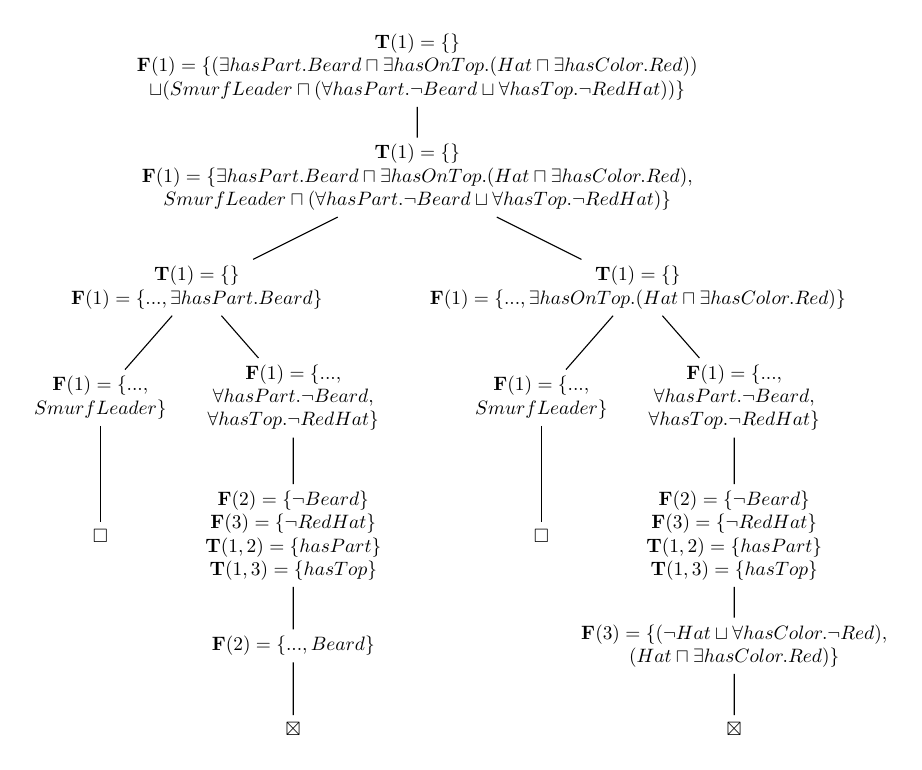
\begin{tikzpicture}[scale=0.7, transform shape,every text node part/.style={align=center},level 1/.style={level distance=2cm},level 2/.style={level distance=2cm, sibling distance=8cm},
level 3/.style={level distance=2cm,sibling distance=3.5cm},level 4/.style={level distance=2.5cm,sibling distance=2cm},level 5/.style={level distance=2cm},level 6/.style={level distance=1.5cm}]
\node [sibling distance=12cm] {$\mathbf{T}(1)=\{\}$ \\ $\mathbf{F}(1)=\{(\exists hasPart.Beard \sqcap \exists hasOnTop.(Hat \sqcap  \exists hasColor.Red))$ \\ $\sqcup (SmurfLeader \sqcap (\forall hasPart.\neg Beard \sqcup \forall hasTop. \neg RedHat)) \}$}
child { node []{$\mathbf{T}(1)=\{\}$ \\ $\mathbf{F}(1)=\{\exists hasPart.Beard \sqcap \exists hasOnTop.(Hat \sqcap  \exists hasColor.Red),$ \\ $SmurfLeader \sqcap (\forall hasPart.\neg Beard \sqcup \forall hasTop. \neg RedHat) \}$}
child { node []{$\mathbf{T}(1)=\{\}$ \\ $\mathbf{F}(1)=\{...,\exists hasPart.Beard  \}$}
	child { node []{$\mathbf{F}(1)=\{...,$\\$SmurfLeader \}$} 
			child{ node {$ \square $}}}
	child { node {$\mathbf{F}(1)=\{...,$\\$\forall hasPart.\neg Beard,$\\$\forall hasTop. \neg RedHat\}$} 
			child{ node[level distance=1cm] {$\mathbf{F}(2)=\{\neg Beard\}$\\$\mathbf{F}(3)=\{\neg RedHat\}$\\$\mathbf{T}(1,2)=\{hasPart\}$\\$\mathbf{T}(1,3)=\{hasTop\}$}
					child{ node[level distance=2cm] {$\mathbf{F}(2)=\{..., Beard\}$}
						   child{ node[level distance=1cm] {$ \boxtimes $}}}}}
}
child { node  []{$\mathbf{T}(1)=\{\}$ \\ $\mathbf{F}(1)=\{..., \exists hasOnTop.(Hat \sqcap  \exists hasColor.Red)\}$}
	child { node {$\mathbf{F}(1)=\{...,$\\$SmurfLeader \}$} 
			child{ node {$ \square $}}}
	child { node {$\mathbf{F}(1)=\{...,$\\$\forall hasPart.\neg Beard,$\\$\forall hasTop. \neg RedHat\}$}
			child{ node[level distance=1cm] {$\mathbf{F}(2)=\{\neg Beard\}$\\$\mathbf{F}(3)=\{\neg RedHat\}$\\$\mathbf{T}(1,2)=\{hasPart\}$\\$\mathbf{T}(1,3)=\{hasTop\}$}
					child{ node[level distance=2cm] {$\mathbf{F}(3)=\{(\neg Hat \sqcup  \forall hasColor.\neg Red),$\\$ (Hat \sqcap  \exists hasColor.Red)\}$}
						   child{ node[level distance=1cm] {$ \boxtimes $}}}} }
}
};

\end{tikzpicture}
\caption{ Le tableau de l'exemple du << Grand Schtroumpf >>. On utilise une règle pour étendre le tableau dans chaque n{\oe}ud.
Dans le premier n{\oe}ud, la règle de la conjonction est appliquée pour $\sqcup$ dans $\mathbf{F}(1)$. Le concept initial est séparé en deux. Ensuite, on applique
la règle de la disjonction pour $\sqcap$ du premier concept dans le deuxième n{\oe}ud. Le tableau est divisé en deux branches. L'expansion est terminée s'il n'y a pas 
de règle applicable ou s'il existe un clash.}\label{grandst}
\end{figure}

Le tableau construit pour l'exemple du << Grand Schtroumpf >> est montré dans la figure \ref{grandst}. Les branches sont étendues séquentiellement. Chaque branche représente une alternative
de modèles. Le symbole $ \boxtimes $ signifie qu'une branche fermée et $ \square $ qu'une branche ouverte. La deuxième branche est fermée à cause d'un clash homogène
détecté dans le modèle 2 ($\neg Beard$ et $Beard$).

Puis, nous pouvons générer un ensemble de concepts non décomposables pour chaque branche ouverte. Un concept qui ne peut subir aucune règle d'expansion est appelé non décomposable.
Dans cet exemple, nous avons deux ensembles:\vspace{-0.2cm}
\begin{align*}
H_1&=\{SmurfLeader,~\exists hasPart.Beard\}\\
H_2&=\{SmurfLeader,~\exists hasOnTop.(Hat \sqcap  \exists hasColor.Red)\}
\end{align*}

Les concepts dans ces deux ensembles sont des éléments pour construire une hypothèse $H$. L'hypothèse $H$ est considérée comme un concept dans $\mathbf{T}(1)$. 
Pour fermer le tableau, on peut prendre ces concepts pour générer un clash hétérogène.
La première branche est fermée si on prend le concept $SmurfLeader$, $\exists hasPart.Beard$ ou la conjonction de ces deux concepts 
$SmurfLeader\sqcap$ $\exists hasPart.$ $Beard$. Le concept $SmurfLeader$ est aussi un concept pour fermer la deuxième branche. On peut alors considérer que $H=SmurfLeader$
est une hypothèse potentielle. A part cette hypothèse, $\exists hasPart.$ $Beard$ $\sqcap \exists hasOnTop.(Hat\sqcap\exists hasColor.Red)$, 
$SmurfLeader\sqcap\exists hasOnTop.(Hat\sqcap \exists hasColor.Red)$, $SmurfLeader \sqcap \exists hasPart.Beard$ sont aussi des hypothèses potentielles.
% Nous pouvons choisir un ensemble $C$ des concepts dans ces ensembles lorsque $C\cap H_i \neq \emptyset$. L'ajout de la conjonction des concepts de $C$ dans $\mathbf{T}()$ peut générer des contradictions dans 
% toutes les branches ouvertes ainsi le tableau est fermé. De ce fait, $C$ est une hypothèse potentielle.

\subsubsection{Fermeture de tableau (ensemble minimal intersectant)}

A ce stade, nous avons réalisé une procédure de construction de l'arbre de la méthode par tableau. Alors on a un ensemble de concepts pour chaque branche ouverte dans le tableau.
Une hypothèse potentielle est la conjonction de ces concepts. Les concepts pris en compte peuvent fermer le tableau si au moins un concept est sélectionné dans chaque branche.
Afin d'éviter la redondance, nous voulons prendre les ensembles minimaux intersectant pour la suite. La définition de l'ensemble intersectant est introduite ci-dessous.
\begin{mydef}{(Ensemble intersectant)}
(Hitting set en anglais). Soit un ensemble non vide:$\{ S_1,\dots,S_n\}$  et $T\subseteq \cup_{i=1}^{n} S_i$. $T$ est un ensemble intersectant pour $\{ S_1,\dots,S_n\}$
si et seulement si  $T \cap S_i \neq \emptyset$ pour tous les $1\leq i\leq n$.
\end{mydef}


Puis, il faut choisir les hypothèses informatives en vérifiant différentes propriétés.
Dans notre situation, une explication est choisie si et seulement si les exigences  suivantes sont vérifiées:
\begin{description}
 \item[\textbf{Inférence}] $\mathcal{K}\vDash \mathcal{H} \sqsubseteq \mathcal{O}$
 \item[\textbf{Cohérence}] $\mathcal{K},\mathcal{H} $ sont cohérents.
 \item[\textbf{Explication}] $\mathcal{K},\nvDash \mathcal{O}, \mathcal{H}   \nvDash \mathcal{O}$
\end{description}
\medskip

Une approche exhaustive est proposée dans l'algorithme~\ref{exhaustive}:

% \begin{algorithm}[H]
% \textbf{Entrée:} Une collection d'ensembles $\{S_1,\dots,S_n\}$\;
% \textbf{Sortie:} Les ensembles intersectants cohérents (Hitting set) $\mathcal{H}$\;
% Initialisation\:
% $\mathcal{H}=\{\}$\;
% Initialisation d'un arbre avec une racine.\;
% \textbf{Pour~}( $i$ De 1 à $n$ )\textbf{~faire:}\\
% ~~~~~~Etendre  les feuilles pour chaque élément de $S_i$  de  chaque feuille actuelle\;
% ~~~~~~Calculer une hypothèse intermédiaire $H_{j}$ de chaque branche $j$: la conjonction de concepts dans la même branche\;
% ~~~~~~Supprimer la branche $j$ si $H_{j}$ n'est pas cohérente par rapport à la base de connaissances\;
% \textbf{Fin Pour}\\
% Pour chaque branche $j$, ajouter l'hypothèse potentielle $H_{j}$: la conjonction de concepts dans la même branche dans $\mathcal{H}$\;
% \textbf{return:} $\mathcal{H}$\;
% \caption{Algorithme pour calculer les ensembles intersectants.}\label{exhaustive}
% \end{algorithm}
\medskip

\begin{figure}
\centering
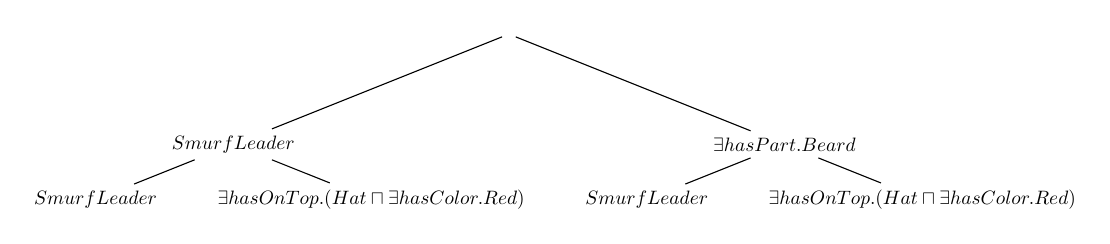
\begin{tikzpicture}[scale=0.7, transform shape, every text node part/.style={align=center},level 1/.style={level distance=2cm,sibling distance=10cm},level 2/.style={level distance=1cm, sibling distance=5cm}]
\node [sibling distance=12cm] {}
child { node []{$SmurfLeader$}
     child{ node []{$SmurfLeader$}}
     child{ node []{$\exists hasOnTop.(Hat \sqcap  \exists hasColor.Red)$}}
}
child { node  []{$\exists hasPart.Beard$}
     child{ node []{$SmurfLeader$}}
     child{ node []{$\exists hasOnTop.(Hat \sqcap  \exists hasColor.Red)$}}
};

\end{tikzpicture}
\caption{L'arbre de la construction d'ensemble intersectant.\label{arbre}}
\end{figure}

Nous illustrons cet algorithme par l'exemple du Schtroumpf. Notons que nous avons obtenu deux ensembles de concepts dans l'étape précédente.
Appliquons cet algorithme, un arbre est initialisé avec une racine. Ensuite, nous construisons récursivement l'arbre en ajoutant les concepts
d'un ensemble $H_i$ dans tous les feuilles de l'arbre. Ici, il y a deux niveaux dans cet arbre (dans la figure \ref{arbre}). Dans ce cas, toutes les
hypothèses sont cohérentes avec TBox. Nous énumérons alors toutes les hypothèses potentielles:
$H=SmurfLeader$, $H=\exists hasPart.Beard \sqcap \exists hasOnTop.(Hat\sqcap\exists hasColor.Red)$, 
$H=SmurfLeader\sqcap\exists hasOnTop.(Hat\sqcap \exists hasColor.Red)$, $H=SmurfLeader \sqcap \exists hasPart.Beard$. La deuxième hypothèse 
est éliminée car $H=\exists hasPart.Beard \sqcap \exists hasOnTop.(Hat\sqcap\exists hasColor.Red)$ n'est pas une hypothèse explicative ($H\vDash \mathcal{O}$). 


Les hypothèses obtenues dans cet algorithme sont cohérentes  et minimales syntaxiquement. Elles sont les conjonctions d'éléments tirés dans chaque branche ouverte.
La cohérence est vérifiée par le service de raisonnement classique de LD.
La minimalité syntaxique est prouvée par l'algorithme des ensembles minimaux intersectants.
La minimalité sémantique doit être considérée afin de choisir la << meilleure >> explication dans notre situation.


\subsection{Minimality criteria}
\textit{Abduction as Inference to the Best Explanation.}
filter inconsistent and redundant ones
% \subsection{Sélection de la meilleure explication selon un critère de minimalité}
Ce que nous obtenons dans l'étape précédente est un ensemble d'hypothèses possibles. Nous ne gardons qu'une partie des hypothèses comme la << meilleure >> explication de l'observation.
Ce choix est défini par un critère de minimalité.


Une hypothèse potentielle est une explication si et seulement si les exigences dans la section précédente sont vérifiées pour éviter les résultats non pertinents et les observations elles-mêmes.
Quand on obtient un ensemble d'hypothèses potentielles, on a besoin
d'un critère de minimalité afin de choisir la << meilleure >> \cite{aliseda1997seeking}.
La simplicité est un critère raisonnable.
Par exemple, $Father \sqcap \exists hasChild.Person \sqsubseteq Man$. le concept $\exists hasChild.Person$ peut être impliqué
à partir du concept $Father$. C'est donc un concept qui porte peu d'information et qu'on peut éliminer pour ne garder que le concept plus simple $Father$. 
La tâche d'interprétation d'une image cérébrale necessite une hypothèse plus générale.
% (i.e. la plus faible explication).

% \begin{mydef}{(La plus faible explication \cite{aliseda1997seeking})}
% $\alpha$ est considérée comme une explication la plus faible pour $\phi$ avec les prémisses $\Theta$ si et seulement si:
% \begin{itemize}
% \item  $\Theta,\alpha \vDash \phi$
% \item  Toutes les autres hypothèses potentielles $\beta$ car $\Theta,\beta \vDash \phi$, on a $\vDash \beta \rightarrow \alpha $
% \end{itemize}
% \end{mydef}

Dans \cite{bienvenu-kr08}, Bienvenu a présenté cinq critères de minimalité utilisés pour l'abduction dans $\mathcal{EL}$.  


Un problème d'abduction est noté $ \langle \mathcal{T}, \mathcal{H}, \mathcal{O}\rangle$, où $\mathcal{T}$ est une TBox, $\mathcal{H}$ est un ensemble de concepts atomiques et $\mathcal{O}$ est un
concept observé.

\begin{mydef}{(Explication~\cite{bienvenu-kr08})}
Soit $\{ A_1,\dots,A_n \} \subseteq \mathcal{H}$ un sous-ensemble de $\mathcal{H}$. Cet ensemble est une explication pour $ \langle \mathcal{T}, \mathcal{H}, \mathcal{O}\rangle$ si et seulement si:
\begin{itemize}
\item  $A_1 \sqcap \dots \sqcap A_n$ est satisfiable dans le cadre de la TBox $\mathcal{T}$.
\item $\mathcal{T}  \vDash  A_1 \sqcap \dots \sqcap A_n \sqsubseteq \mathcal{O}$
\end{itemize}

\end{mydef}


\begin{mydef}{(Critères de minimalité~\cite{bienvenu-kr08})}
Soit un problème d'abduction $\mathcal{P}=\langle \mathcal{T},\mathcal{H}, \mathcal{O}\rangle$,$\mathcal{A}=\{H_1,\dots,$ $H_n \} \subseteq \mathcal{H}$ une explication du problème $\mathcal{P}$,
$\langle H_{(1)},\dots,H_{(n)}\rangle$ un ordre de priorité sur $\mathcal{H}$,
et $w:\mathcal{H}\rightarrow \mathbb{N}$ une fonction affectant une valeur d'importance à un concept. On peut formuler différents critères comme:
% \begin{itemize}
% \item  $\mathcal{A}~$ est  $~\subseteq -minimal$ s'il n'existe pas d'explication $\mathcal{B}$ pour $\mathcal{P}$ telle que $\mathcal{B} \subsetneq \mathcal{A}$,
% \item  $\mathcal{A}~$ est  $~\leq -minimal$ s'il n'existe pas d'explication $\mathcal{B}$ pour $\mathcal{P}$ telle que $\abs{\mathcal{B}} < \abs{\mathcal{A}}$,
% \item  $\mathcal{A}~$ est  $~\subseteq_P -minimal$ s'il n'existe pas d'explication $\mathcal{B}$ pour $\mathcal{P}$ telle que $\mathcal{B} \cap H_i \subsetneq \mathcal{A}\cap H_i$ et
% $\mathcal{B} \cap H_j = \mathcal{A}\cap H_j$ lorsque $1\leq j< i$,
% \item  $\mathcal{A}~$ est  $~\leq_P -minimal$ s'il n'existe pas d'explication $\mathcal{B}$ pour $\mathcal{P}$ telle que $\abs{\mathcal{B} \cap H_i} < \abs{\mathcal{A}\cap H_i}$ et
% $\abs{\mathcal{B} \cap H_j} = \abs{\mathcal{A}\cap H_j}$ lorsque $1\leq j< i$,
% \item  $\mathcal{A}~$ est  $~\sqsubseteq_w -minimal$ s'il n'existe pas d'explication $\mathcal{B}$ pour $\mathcal{P}$ telle que $\sum_{B \in \mathcal{B}}w(B) < \sum_{A \in \mathcal{A}}w(A)$.
% \end{itemize}
 \end{mydef}



Un autre critère spécifique est mentionné pour une application de << matchmaking >> dans~\cite{DiNoia07}.
Comme dans les travaux de Colucci, l'explication est alors la conjonction de concepts manquant par rapport à l'observation. Dans \cite{DiNoia07},
les auteurs ont proposé un critère irréductible-minimal dans leur formalisme. 
Une solution irréductible est un concept sous  forme  normale conjonctive lorsqu'il n'y a pas d'autre solution qui est un sous-concept de la solution irréductible.

En fait une explication irréductible est un sous-ensemble de concepts de l'observation. Une explication irréductible est la conjonction de concepts atomiques
qui n'apparaissent pas dans la contrainte mais dans l'observation. 
Ce modèle de l'explication est approprié pour une application de matchmaking mais c'est une explication avec peu d'information pour notre cas traditionnel.

Nous pouvons cependant adapter ce critère à notre problème. Nous pouvons alors calculer la cardinalité du résultat irréductible pour la comparaison.
On peut représenter les concepts sous forme normale conjonctive (FNC) pour les hypothèses et l'observation. Comme l'hypothèse est subsumée par l'observation, les concepts conjonctifs de l'hypothèse sont un sous-ensemble
de ceux de l'observation. On présente une fonction métrique $f_{ranking}$ pour évaluer la qualité cette hypothèse. Ici, on peut calculer la cardinalité de la partie différente
entre l'hypothèse et l'observation. Le concept avec le moins de différence par rapport aux autres hypothèses est préféré comme une explication minimale irréductible. On peut aussi
assigner une valeur à chaque concept et calculer la pondération pour  la partie différente.


\begin{mydef}{(Critère de subsomption et irréductibilité)}
Soit un problème d'abduction $\mathcal{P}=\langle \mathcal{T},\mathcal{H}, \mathcal{O}\rangle$, et $\{\langle P_{1},\dots,P_{n}\rangle\}$ les explications potentielles. 
On peut formuler différents critères comme:
% \begin{itemize}
% \item  $P_{i}$ est une explication suivant le critère de subsomption $\bm{\sqsubseteq -minimal}$ s'il n'existe pas d'explication $P_{j}$ pour $\mathcal{P}$ tel que $P_{i}\sqsubseteq P_{j}$
% \item  $P_{i}$ est une explication irréductible $\bm {irreductible-minimal }$ s'il n'existe pas d'explication $P_{j}$ pour $\mathcal{P}$ tel que $f_{ranking}(\mathcal{T},FNC(P_{j}),FNC(\mathcal{O})) 
% < f_{ranking}(\mathcal{T},FNC(P_{i}),FNC(\mathcal{O}))$
% \end{itemize}

\end{mydef}


Les critères introduits par Bienvenu sont utiles lorsqu'une hypothèse ne contient que les concepts atomiques. Elle considère qu'une hypothèse est construite par la conjonction de certains concepts atomiques.
Le critère bénéficie de la relation entre les ensembles. Dans notre problème, une hypothèse peut être composée par des concepts non atomiques. Le critère de subsomption est un bon choix dans plusieurs travaux,
par exemple, ceux de Colucci et al.~\cite{colucci2004uniform} et ceux de Atif et al.~\cite{jamal13}. La relation hiérarchique est prise en compte pour chercher une hypothèse plus générale.
Le critère d'irréductibilité est un critère combinant un critère de subsomption et un critère de cardinalité. Ce critère a l'avantage que la mesure $f_{ranking}$ est modifiable en fonction du besoin.
Par exemple, si on applique l'abduction dans la logique floue, un degré de possibilité peut être considéré comme une mesure pratique. Dans le cadre du stage, nous n'avons pas évaluer la coefficient de priorité
de concepts. Nous considérons les concepts sont équilibrés et utilisons les critères d'inclusion, de cardinalité, de subsomption et d'irréductibilité pour la suite.




\subsection{Résultats, évaluation et discussion}
Notre approche est implémentée en Java en utilisant les librairies OWL API\footnote{\url{http://owlapi.sourceforge.net/}} et Pellet\footnote{\url{http://clarkparsia.com/pellet/}}.
OWL est une API\footnote{application programming interface en anglais} open-source de Java sous licence de LGPL. 
Elle permet de créer, de manipuler l'ontologie. Une interface entre l'ontologie et la logique de description est mise en {\oe}uvre aussi.
Pellet est un moteur d'inférence gratuit pour fournir les services de raisonnement comme les tests de satisfiabilité et subsomption.
Dans notre projet,  la base de connaissances et l'observation sont codées en ontologie avec le logiciel << The Protégé >>\footnote{\url{http://protege.stanford.edu/}}.
Nous réalisons la méthode par tableau par la structure d'arbre qui permet de construire un tableau et la structure d'ensemble qui permet de
manipuler les ensembles de concepts. Les règles d'expansion et les détections de contradictions sont implémentées avec l'aide des deux librairies pour développer le tableau.

\subsubsection{Deux exemples d'abduction par la méthode par tableau adapté proposée}
\label{exemples}
Le premier exemple est un test de l'interprétation d'images cérébrales.
Pour tester la procédure proposée dans le cadre de l'interprétation d'images cérébrales, nous commençons
par construire un morceau de la base de connaissances et formuler l'observation manuellement.
Voici la TBox pour représenter la connaissance et l'observation obtenue:\vspace{-0.3cm}
\begin{align*}
\mathcal{T}=\{~SmallDeformingTumor &\sqsubseteq BrainTumor\\
 &~~~~~\sqcap \exists hasEnhancement. NonEnhanced \\
&~~~~~\sqcap \exists hasBehavior. Infiltrating  \\
PeripheralDeformingTumor &\sqsubseteq BrainTumor\\
&~~~~~ \sqcap \exists farFrom. LateralVentricle \\
&~~~~~ \sqcap \exists hasLocation. PeripheralCerebralHemisphere \} 
\end{align*}\vspace{-0.9cm}
\begin{align*}
\mathcal{O} =\{&~\exists hasEnhancement. NonEnhanced \\
 &\sqcap \exists farFrom. LateralVentricle \\
&\sqcap \exists hasLocation. PeripheralCerebralHemisphere \} 
\end{align*}

Dans ce cas, il n'y a pas de contrainte. Le n{\oe}ud initial est donc $\mathbf{T}(1)=\{\}, \mathbf{F}(1)=\{\neg C_\mathcal{T}\sqcap \mathcal{O}\}$.
\footnote{Les concepts et les rôles sont représentés abrégés ici.}\vspace{-0.3cm}
\begin{align*}
 \neg C_\mathcal{T}\sqcap \mathcal{O}= \{ &(SDT \sqcap \neg BT \sqcup \forall hE. \neg NE \sqcup \forall hB. \neg In) \sqcup \\
 &(PDT \sqcap \neg BT \sqcup \forall fF. \neg LV \sqcup \forall hL. \neg PCH) \sqcup \\
 &(\exists hE. NE \sqcap \exists fF. LV \sqcup \exists hL.PCH )\}
\end{align*}
% \footnote{Le tableau d'expansion est montré dans l'annexe.}
Par la méthode de tableau, il reste six branches ouvertes. Dans chaque branche, on a un ensemble de concepts
non décomposables:\vspace{-0.25cm}
 \begin{align*}
  H_1&=\{ SDT, PDT, \exists hE.NE\}\\
  H_2&=\{ SDT, PDT, \exists fF.LV\}\\
  H_3&=\{ SDT, PDT, \exists hL.PCH\}\\
  H_4&=\{ SDT, \neg BT, \forall fF. \neg LV, \forall hL. \neg PCH, \exists hE.NE\}\\
  H_5&=\{ PDT, \neg BT, \forall hE. \neg NE, \forall hB. \neg In, \exists fF.LV\}\\
  H_6&=\{ PDT, \neg BT, \forall hE. \neg NE, \forall hB. \neg In, \exists hL.PCH\}\\
 \end{align*}\vspace{-0.9cm}

Ensuite, on utilise l'algorithme exhaustif pour générer les hypothèses potentielles.
On choisit un concept de chaque ensemble. Une hypothèse est la conjonction de ces concepts.
En même temps, les hypothèses incohérentes sont éliminées, par exemple $SDT \sqcap \neg BT$, 
$PDT \sqcap \forall fF \neg LV$, etc. L'hypothèse $\exists hE. NE \sqcap \exists fF. LV \sqcup \exists hL.PCH $
est éliminée. Cette hypothèse est peu informative parce qu'elle est subsumée par l'observation sans la base de connaissances.

En appliquant le critère de subsomption, les hypothèses $SDT \sqcap \exists fF.LV \sqcap \exists hL.PCH$
et $PDT \sqcap \exists hE.NE$ sont considérées comme les explications. Par exemple, une hypothèse potentielle
$SDT \sqcap PDT$ est subsumée par ces deux explications. Ces deux résultats sont confirmés par les propriétés
de cohérence, d'explication et de minimalité. Nous obtenons alors deux bonne explications de cette observations:
\begin{itemize}
 \item $PeripheralDeformingTumor \sqcap \exists hasEnhancement. NonEnhanced$
 \item $SmallDeformingTumor\sqcap \exists farFrom. LateralVentricle $\\ $\sqcap \exists hasLocation. PeripheralCerebralHemisphere$
\end{itemize}

\medskip

Le deuxième exemple est extrait de~\cite{klarman2011abox}:\vspace{-0.25cm}
\begin{align*}
 \mathcal{T}=\{~~&Optimist \sqcup (Nihilist\sqcap \exists owns.Dog)\sqsubseteq Happy\\
~~&\forall watches.Comedy \sqsubseteq Optimist \}\\ 
\mathcal{A}=\{~~&Nihilist(John),~Dog(Snoopy)\}\\
\mathcal{O}=~~~~~&Happy(john).
\end{align*}

C'est un problème d'abduction de ABox. Nous pouvons le transformer en un problème d'abduction de concept.
L'observation est représentée par le concept $Happy$.
Les assertions dans l'ABox sont considérées comme les contraintes, 
alors le n{\oe}ud initial est $\mathbf{T}(1)=\{Nihilist\},\mathbf{T}(2)=\{Dog\}, \mathbf{F}(1)=\{\neg C_\mathcal{T}\sqcap Happy\}$
On peut construire un tableau et vérifier les clashs dans toutes les branches\footnote{Le tableau est décrit dans l'annexe \ref{C}.}. Il n'y a qu'une branche ouverte. L'ensemble des concepts non décomposables est:\vspace{-0.2cm}
$$H_1=\{Happy, \forall watches.Comedy, Optimist, \exists own.Dog\}$$
On peut prendre un concept comme une hypothèse potentielle. Mais le concept $Happy$ est éliminé parce qu'il est équivalent avec l'observation. De plus, $\forall watches.Comedy \sqsubseteq Optimist$. Le concept $\forall watches.Comedy$ ne peut pas être considéré comme une explication en prenant en compte le critère de subsomption. 
Les concepts $Optimist$ et $ \exists own.Dog$ sont donc deux << meilleures >> explications.

Les résultats de ces deux exemples montrent que notre approche permet de trouver une explication considérant 
le critère de minimalité. Les explications sont cohérentes et explicatives.  Notre approche est capable de
retrouver la présence d'une pathologie disposant une petite base de connaissances. Dans le  résultat du deuxième 
exemple, nous pouvons trouver les mêmes explications que dans \cite{klarman2011abox} en donnant les assertions des concepts
avec l'individu $John$. De plus, nous utilisons le critère de minimalité pour sélectionner la << meilleure >> explication.
Dans les travaux de \cite{colucci2004uniform} et \cite{EKMRMW07},  la TBox est limitée puisque la partie gauche d'un axiome ne peut contenir qu'un concept simple. Nous pouvons mettre un concept complexe  sans ajouter d'autres axiomes.
Notre approche est adatptée à la TBox générale du langage $\mathcal{ALC}$.

\subsubsection{Comparaison des critères de minimalité}
Dans cette section, on compare les différents critères sur l'exemple du Schtroumpf.

% \begin{figure}[h]
% \begin{center}
% \includegraphics[width=0.7\textwidth]{4smurf.png}
% \caption{Les Schtroumpfs.\label{4smurf}}
% \end{center}
% \end{figure}

D'après les personnages et leur habillement, on peut formuler une base de connaissances comme ci-dessous:\vspace{-0.3cm}
\begin{align*}
\mathcal{T}=\{ SmurfLeader &\sqsubseteq Smurf \sqcap \exists hasPart.Beard \sqcap \exists hasOnTop.RedHat. \\
SmurfFollower &\sqsubseteq Smurf \sqcap \exists hasOnTop.WhiteHat. \\
SmurfFemale &\sqsubseteq Smurf \sqcap \exists hasOnTop.WhiteHat \sqcap \exists hasPart.GoldenHair. \\
RedHat &\equiv Hat \sqcap \exists hasColor.Red. \\
WhiteHat &\equiv Hat \sqcap \exists hasColor.White. \\
GoldenHair &\equiv Hair \sqcap \exists hasColor.Golden.\}
\end{align*}
\paragraph*{Première observation}

Si on a une image dont un chapeau blanc est segmenté, on peut alors la représenter par un concept:\vspace{-0.1cm}
$$\mathcal{O}= \exists hasOnTop.(Hat \sqcap \exists hasColor.White).$$

En appliquant l'algorithme de tableau sémantique qu'on a proposé, on a deux branches ouvertes à la fin:
\begin{itemize}
 \item $\{ \exists hasOnTop.WhiteHat, SmurfLeader, SmurfFollower,SmurfFemale\}$
 \item $\{ \neg Smurf, \forall hasOnTop. \neg RedHat, \forall hasPart.\neg Beard, \forall hasOnTop. WhiteHat, \\ SmurfFollower,SmurfFemale\}$
\end{itemize}
\medskip

On doit choisir un concept ou la conjonction de plusieurs concepts pour fermer les deux branches ouvertes. L'hypothèse qu'on a choisie doit 
respecter les exigences mentionnées dans la première section.

Par exemple, le concept $SmurfFollower$ existe dans les deux branches, donc c'est une hypothèse potentielle qui vérifie $\mathcal{K}\vDash \mathcal{H} \sqsubseteq \mathcal{O}$.
De plus, c'est cohérent avec la TBox et explicatif car $\mathcal{K} \nvDash \mathcal{O}, \mathcal{H}   \nvDash \mathcal{O}$.

En revanche, si on prend $SmurfLeader \sqcap \forall hasOnTop. \neg RedHat$, c'est une hypothèse incohérente donc elle n'est pas prise en compte. 
Si on choisit $\exists hasOnTop.WhiteHat \sqcap \forall  hasOnTop.WhiteHat$, c'est une hypothèse non explicative donc elle n'est pas prise en compte non plus.

Les résultats préférés sont:

(Inclusion de l'ensemble): $SmurfFollower$, $SmurfFemale$

(Cardinalité): $SmurfFollower$, $SmurfFemale$

(Irréductibilité): $SmurfFollower$

(Subsomption): $SmurfFollower$
\paragraph*{Deuxième observation}

Si on a une image du deuxième schtroumpf dans  la figure \ref{4smurf}, on peut alors segmenter son chapeau et ses lunettes avec des outils de traitement d'images.
Le concept de l'observation est représenté comme:
\begin{align*}
\mathcal{O}= \exists hasOnTop.(Hat \sqcap \exists hasColor.White) \sqcap \exists hasPart.Glasses.
\end{align*}

 Les résultats préférés sont:
 
(Inclusion de l'ensemble): $SmurfFollower \sqcap \exists hasPart.Glasses$, $SmurfFemale \sqcap \exists hasPart.Glasses$

(Cardinalité): $ SmurfFollower \sqcap \exists hasPart.Glasses$ , $ SmurfFemale \sqcap \exists hasPart.Glasses$

(Irréductibilité): $ SmurfFollower \sqcap \exists hasPart.Glasses$

(Subsomption): $SmurfFollower \sqcap \exists hasPart.Glasses$

Le critère d'inclusion et le critère de cardinalité ne sont pas suffisants pour décider la << meilleure >> explication dans ce contexte.
La relation hiérarchique entre les concepts n'est pas prise en compte.
En particulier, ces deux critères sont souvent utilisés quand le résultat est composé de concepts atomiques.
\paragraph*{Troisième observation}
Si on prend la première observation et on modifie la TBox comme ci-dessous:\vspace{-0.3cm}
\begin{align*}
\mathcal{T}=\{ SmurfLeader &\sqsubseteq Smurf \sqcap \exists hasPart.Beard \sqcap \exists hasOnTop.RedHat. \\
SmurfEtudiant &\sqsubseteq Smurf \sqcap \exists hasOnTop.WhiteHat \sqcap \exists hasPart.Glasses. \sqcap \exists hasInHand.Book \\
SmurfFemale &\sqsubseteq Smurf \sqcap \exists hasOnTop.WhiteHat \sqcap \exists hasPart.GoldenHair. \\
RedHat &\equiv Hat \sqcap \exists hasColor.Red. \\
WhiteHat &\equiv Hat \sqcap \exists hasColor.White. \\
GoldenHair &\equiv Hair \sqcap \exists hasColor.Golden.\}
\end{align*}

Les résultats préférés sont:

(Inclusion de l'ensemble): $SmurfEtudiant$, $SmurfFemale$

(Cardinalité): $SmurfEtudiant$, $SmurfFemale$
 
(Irréductibilité): $SmurfFemale$

(Subsomption): $SmurfEtudiant$, $SmurfFemale$

Évidemment, la << meilleure >> explication est la disjonction de $SmurfEtudiant$ et $SmurfFemale$, que l'on peut associer à un concept $SmurfFollower$ mais qui n'a pas d'axiome dans
cette base de connaissances. L'algorithme qu'on propose ne permet pas de générer une explication avec des disjonctions. C'est une limite de notre approche. 

Les critères d'inclusion de l'ensemble et de la cardinalité ne sont pas assez bons par rapport aux critères de l'irréductibilité et la subsomption, puisque la relation hiérarchique entre les concepts
 n'est pas prise en compte. Ils sont adaptés aux hypothèses construites par la conjonction de certains concepts atomiques.
Pour le problème actuel, le critère de l'irréductibilité contient la préférence de la subsomption et la préférence de la cardinalité. 
Nous observons que les critères de subsomption et d'irréductibilité sont bien meilleurs sur notre situation.


\section{Perspectives}\label{sec:persp}
Several directions will be presented in this section:
\begin{itemize}
 \item concrete domain with fuzzy logic.
 Concrete domains are necessary when semantic truth concept has no corresponding space in concrete domain.
 \item how to generate potential hypotheses.
 \item how to select the ``best'' explanation with an appropriate minimality criterion.
 \item perspective of publications.
\end{itemize}

\section{Activities}
\begin{itemize}
 \item project LOGIMA
 \item seminars
 \item doctoral formation
\end{itemize}

% \nocite{*}
\bibliographystyle{plain}
\bibliography{mi_ref}
\end{document}


% \section{Tableaux method}
% First of all, we recall the expansion rules of the tableau method in $\mathcal{ALCI_{R_+}}$.
% 
% \begin{mydef}($\mathcal{ALCHI_{R+}}$ tableau)
% Let $D$ be an $\mathcal{ALC}$ concept in NNF and let $R_D$ be the set of roles in $\mathcal{ALC}$, a tableau $T$ for $D$ is defined as a triple $(\mathbf{S},\mathcal{L}, \mathcal{E})$, 
% where $\mathbf{S}$ is a set of interpretation elements; 
% $\mathcal{L}$ relates each interpretation element to a set of concepts occurring in $D$ (from $\mathbf{S}$ to $\mathcal{P}(\mathfrak{C}$)); 
% $\mathcal{E}$ relates each pair of interpretation elements to a set of roles in $R_D$  (from $\mathbf{S}\times\mathbf{S}$ to $\mathcal{P}(R_D)$). 
% 
% The decision procedure to check the satisfiability of a given concept $D$ is based on constructing a model using the tableau method. 
% Let $x$ and $y$ be two interpretation elements in $\mathbf{S}$ ($x,~y\in \mathbf{S}$), $C,E$ be two concepts occurring in $D$ and $r\in R_D$.
% The model is constructed as a tree structure where each node corresponds to an element of interpretation $x\in \Delta^\mathcal{I}$.
% The node is labeled with a set of concepts $\mathcal{L}(x)$.
% The edge between the nodes $x$ and $y$ is labeled with corresponding roles $r\in\mathcal{E}(\langle x,y \rangle)$.
% The following conditions hold:
% \begin{itemize}
% \item if $C\in \mathcal{L}(x)$, then $\neg C\notin\mathcal{L}(x)$.
% \item if $C\sqcap E\in \mathcal{L}(x)$, then $ C\in\mathcal{L}(x)$ and $ E\in\mathcal{L}(x)$.
% \item if $C\sqcup E\in \mathcal{L}(x)$, then $ C\in\mathcal{L}(x)$ or $ E\in\mathcal{L}(x)$.
% \item if $\exists r.C\in \mathcal{L}(x)$, then there exists some $y\in \mathbf{S}$  such that $r \in \mathcal{E}(\langle x,y\rangle)$ and $C\in\mathcal{L}(y)$.
% \item if $\forall r.C\in \mathcal{L}(x)$, then for all  existing $y \in \mathbf{S}$ such that $r \in \mathcal{E}(\langle x,y\rangle)$, $C\in\mathcal{L}(y)$.
% \item if $\forall r.C\in \mathcal{L}(x)$, $r \in \mathcal{E}(\langle x,y\rangle)$ and $r$ is a transitive role, then $\forall r.C\in \mathcal{L}(y)$.
% \item if $\forall r.C\in \mathcal{L}(x)$, $v \in \mathcal{E}(\langle x,y\rangle)$, $v\sqsubseteq r$ (or $v^-\sqsubseteq r^-$) and $v$ is a transitive role, then $\forall v.C\in \mathcal{L}(y)$.
% \item $r \in \mathcal{E}(\langle x,y\rangle)$ iff  $ r^-\in \mathcal{E}(\langle y,x\rangle)$.
% \item $ r\in \mathcal{E}(\langle x,y\rangle)$ and $r\sqsubseteq v$ (or $r^-\sqsubseteq v^-$) then  $v \in \mathcal{E}(\langle x,y\rangle)$.
% \end{itemize}
% \end{mydef}
% \section{Example}
%  The complete knowledge base is given as follows:
% \begin{align*}
%  TBox=\{ Hemisphere &\sqsubseteq \exists isPartOf. Brain\\
% 	 BrainStructure &\sqsubseteq \exists isPartOf. Brain\\
% 	 BrainDisease &\sqsubseteq \exists isPartOf. Brain \sqcap \neg BrainStructure\\
% 	 Tumor  &\sqsubseteq BrainDisease\\
% 	 LVl &\sqsubseteq BrainStructure \sqcap \exists (rightOf \sqcap closeTo). CNl\\
% 	 LVr &\sqsubseteq BrainStructure \sqcap \exists (leftOf \sqcap closeTo). CNr\\
% 	 CNl &\sqsubseteq BrainStructure\\
% 	 CNr &\sqsubseteq BrainStructure\}
% % 	 WMl &\sqsubseteq BrainStructure\\
% % 	 WMr &\sqsubseteq BrainStructure\\
% % 	 PUl &\sqsubseteq BrainStructure\\
% % 	 PUr &\sqsubseteq BrainStructure\\
% % 	 THl &\sqsubseteq BrainStructure\\
% % 	 THr &\sqsubseteq BrainStructure\}
% \end{align*}
% The role axioms are described as:
% \begin{align*}
%  RBox=\{ rightOf &\equiv leftOf^-\\
%          above &\equiv below^- \\
% 	 closeTo &\equiv closeTo^- \\
% 	 farFrom &\equiv farFrom^- \\
% 	 isPartOf \circ isPartOf &\sqsubseteq isPartOf \\
% 	 hasPart \circ hasPart &\sqsubseteq hasPart\\
% 	 isPartOf &\equiv hasPart^-\}
% \end{align*}
% 
% % The ABox is used for describing the observation in the image.
% % The spatial configuration describes the relationships between different structures.
% The ABox represents the observation of recognized structures and the relationships with others.
% For example, a region is recognized as the left caudate nucleus (CNl), denoted by $a$.
% The region of brain is denoted by $c$. An unknown region is segmented and their relationships are computed.  
% Such an observation can be represented as
% % \footnote{At first, I assume to use a threshold to convert quantification measures to qualitative representations. However, the threshold 
% % is hard to choose. If we use a fuzzy ABox, only the spatial relations are assigned with a satisfaction degree. However, I have not read the reference about reasoning service on fuzzy Description Logics yet.}:
% \begin{align*}
%  ABox=\{ a&: CNl \\
% 	 b&: unknown \\
% 	 c&: Brain \\
% 	 \langle a,b\rangle &: leftOf, closeTo \\
% 	 \langle b,c\rangle &: isPartOf\}
% \end{align*}
% 
% % In an image understanding application, we reason about a description which explains a given image in a certain domain.
% In this example, the ABox describes an observation of a given scene and the objective is to find a reasonable description of  the unknown object $b$.
% % This type of reasoning can be treated as an abductive reasoning.
% A possible hypothesized description is $LVl\sqcap \exists isPartOf.Hemisphere$.
% The hypothesis can be verified by a concept subsumption checking: $\mathcal{K} \vDash H\sqsubseteq O$, where $H$ is the explained concept for the observation $O$.
% To check subsumption of two concepts $H$ and $O$, $\mathcal{K} \vDash H\sqcap \neg O \sqsubseteq \bot$ is required to prove that $H\sqcap \neg O$ is unsatisfiable.
% 
% In this example, $O\equiv \exists (leftOf^-\sqcap closeTo^-).CNl\sqcap \exists isPartOf.Brain$ and $H\equiv LVl\sqcap \exists isPartOf.Hemisphere$.
% Let $x$ be the interpretation element of the concept $H\sqcap \neg O$. 
% 
% The tableau is initialized with $\mathcal{L}(x)=\{ LVl\sqcap \exists isPartOf.Hemisphere\sqcap \forall (leftOf^-\sqcap closeTo^-).CNl\sqcup \forall isPartOf.\neg Brain\}$.
% The $\sqcap$, $\sqcup$ rules are applied and we obtain:
% \begin{center}
% \begin{tikzpicture}[every text node part/.style={align=center},level 1/.style={level distance=1.5cm, sibling distance=9cm}]
% \node [sibling distance=18cm] {$\mathcal{L}(x)=\{ LVl\sqcap \exists isPartOf.Hemisphere\sqcap \forall (leftOf^-\sqcap closeTo^-).CNl\sqcup \forall isPartOf.\neg Brain\}$}
% 	      child{ node {$\mathcal{L}(x)=\{ LVl,~\exists isPartOf.Hemisphere,$\\$~\forall (leftOf^-\sqcap closeTo^-).\neg CNl\}$}}
% 	      child{ node {$\mathcal{L}(x)=\{ LVl,~\exists isPartOf.Hemisphere,$\\$~\forall isPartOf.\neg Brain\}$}};
% \end{tikzpicture} 
% \end{center}
% 
% To integrate terminological knowledge, axioms in the form $C\sqsubseteq D$ in TBox can be internalized into single concepts ($\neg C\sqcup D$) and added to $\mathcal{L}(x)$. Here, for the sake of simplicity 
% of demonstration, we only add the internalization of the axiom $LVl \sqsubseteq BrainStructure \sqcap  \exists (rightOf \sqcap closeTo). CNl$ for the first branch.
% \begin{center}
% \begin{tikzpicture}[every text node part/.style={align=center},level 1/.style={level distance=1.5cm, sibling distance=9cm}]
% \node [sibling distance=18cm] {$\mathcal{L}(x)=\{ LVl\sqcap \exists isPartOf.Hemisphere\sqcap \forall (leftOf^-\sqcap closeTo^-).CNl\sqcup \forall isPartOf.\neg Brain\}$}
% 	      child{ node {$\mathcal{L}(x)=\{ LVl,~\exists isPartOf.Hemisphere,$\\$~\forall (leftOf^-\sqcap closeTo^-).\neg CNl,$\\$\neg LVl \sqcup BrainStructure \sqcap \exists (rightOf \sqcap closeTo).CNl\}$}}
% 	      child{ node {$\mathcal{L}(x)=\{ LVl,~\exists isPartOf.Hemisphere,$\\$~\forall isPartOf.\neg Brain\}$}};
% \end{tikzpicture}  
% \end{center}
% 
% We then apply $\sqcup$ and $\sqcap$ rules again on the first branch:
% \begin{center}
% \begin{tikzpicture}[every text node part/.style={align=center},level 1/.style={level distance=1.5cm, sibling distance=9cm}, level 2/.style={level distance=2cm, sibling distance=6cm}]
% \node [sibling distance=18cm] {$\mathcal{L}(x)=\{ LVl\sqcap \exists isPartOf.Hemisphere\sqcap \forall (leftOf^-\sqcap closeTo^-).\neg CNl\sqcup \forall isPartOf.\neg Brain\}$}
% 	      child{ node {$\mathcal{L}(x)=\{ LVl,~\exists isPartOf.Hemisphere,$\\$~\forall (leftOf^-\sqcap closeTo^-).\neg CNl,$\\$\neg LVl \sqcup BrainStructure \sqcap \exists (rightOf \sqcap closeTo).CNl\}$}
% 	      		    child{ node {$\mathcal{L}(x)=\{ LVl,~\exists isPartOf.Hemisphere,$\\$~\forall (leftOf^-\sqcap closeTo^-).\neg CNl,$\\$\neg LVl\}$}
% 				  child{ node{$\boxtimes$}}}
% 		            child{ node {$\mathcal{L}(x)=\{ LVl,~\exists isPartOf.Hemisphere,$\\$~\forall (leftOf^-\sqcap closeTo^-). \neg CNl,$\\$BrainStructure,$\\$\exists (rightOf \sqcap closeTo).CNl$}}}
% 	      child{ node {$\mathcal{L}(x)=\{ LVl,~\exists isPartOf.Hemisphere,$\\$~\forall isPartOf.\neg Brain\}$}};
% \end{tikzpicture}  
% \end{center}
% 
% A clash ($LVl,~\neg LVl$) is detected in the first part of the first branch (closed). We then apply $\exists$ on the second part:
% \begin{center}
% \begin{tikzpicture}[every text node part/.style={align=center},level 1/.style={level distance=1.5cm, sibling distance=9cm}, level 2/.style={level distance=2cm, sibling distance=6cm},
% level 3/.style={level distance=2.5cm, sibling distance=6cm}]
% \node [sibling distance=18cm] {$\mathcal{L}(x)=\{ LVl\sqcap \exists isPartOf.Hemisphere\sqcap \forall (leftOf^-\sqcap closeTo^-).\neg CNl\sqcup \forall isPartOf.\neg Brain\}$}
% 	      child{ node {$\mathcal{L}(x)=\{ LVl,~\exists isPartOf.Hemisphere,$\\$~\forall (leftOf^-\sqcap closeTo^-).\neg CNl,$\\$\neg LVl \sqcup BrainStructure \sqcap \exists (rightOf \sqcap closeTo).CNl\}$}
% 	      		    child{ node {$\mathcal{L}(x)=\{ LVl,~\exists isPartOf.Hemisphere,$\\$~\forall (leftOf^-\sqcap closeTo^-).\neg CNl,$\\$\neg LVl\}$}
% 				  child{ node{$\boxtimes$}}}
% 		            child{ node {$\mathcal{L}(x)=\{ LVl,~\exists isPartOf.Hemisphere,$\\$~\forall (leftOf^-\sqcap closeTo^-).\neg CNl,$\\$BrainStructure,$\\$\exists (rightOf \sqcap closeTo).CNl$}
% 				  child{ node {$\mathcal{L}(x)=\{ LVl,~\exists isPartOf.Hemisphere,$\\
% 				  $~\forall (leftOf^-\sqcap closeTo^-).\neg CNl,$\\$BrainStructure,$\\$\exists (rightOf \sqcap closeTo).CNl$\\
% 				  $\mathcal{L}(y)=\{CNl\}$\\
% 				  $\mathcal{E}(\langle x,y \rangle)=\{rightOf,closeTo\}$}}}}
% 	      child{ node {$\mathcal{L}(x)=\{ LVl,~\exists isPartOf.Hemisphere,$\\$~\forall isPartOf.\neg Brain\}$}};
% \end{tikzpicture}  
% \end{center}
% 
% Because of inverse role axioms in RBox, we can add inverse roles in $\mathcal{E}(\langle x,y \rangle)$ and apply  $\forall$ rule on the second part:
% \begin{center}
% \begin{tikzpicture}[every text node part/.style={align=center},level 1/.style={level distance=1.5cm, sibling distance=9cm}, level 2/.style={level distance=2cm, sibling distance=6cm},
% level 3/.style={level distance=2.5cm, sibling distance=6cm}]
% \node [sibling distance=18cm] {$\mathcal{L}(x)=\{ LVl\sqcap \exists isPartOf.Hemisphere\sqcap \forall (leftOf^-\sqcap closeTo^-).\neg CNl\sqcup \forall isPartOf.\neg Brain\}$}
% 	      child{ node {$\mathcal{L}(x)=\{ LVl,~\exists isPartOf.Hemisphere,$\\$~\forall (leftOf^-\sqcap closeTo^-).\neg CNl,$\\$\neg LVl \sqcup BrainStructure \sqcap \exists (rightOf \sqcap closeTo).CNl\}$}
% 	      		    child{ node {$\mathcal{L}(x)=\{ LVl,~\exists isPartOf.Hemisphere,$\\$~\forall (leftOf^-\sqcap closeTo^-).\neg CNl,$\\$\neg LVl\}$}
% 				  child{ node{$\boxtimes$}}}
% 		            child{ node {$\mathcal{L}(x)=\{ LVl,~\exists isPartOf.Hemisphere,$\\$~\forall (leftOf^-\sqcap closeTo^-).\neg CNl,$\\$BrainStructure,$\\$\exists (rightOf \sqcap closeTo).CNl$}
% 				  child{ node {$\mathcal{L}(x)=\{ LVl,~\exists isPartOf.Hemisphere,$\\
% 				  $~\forall (leftOf^-\sqcap closeTo^-).\neg CNl,$\\$BrainStructure,$\\$\exists (rightOf \sqcap closeTo).CNl$\\
% 				  $\mathcal{L}(y)=\{CNl,~\neg CNl\}$\\
% 				  $\mathcal{E}(\langle x,y \rangle)=\{rightOf,closeTo,leftOf^-,closeTo^-\}$\\
% 				  $\mathcal{L}(y,x)=\{rightOf^-,closeTo^-,leftOf,closeTo\}$}
% 				  child{ node{$\boxtimes$}}}}}
% 	      child{ node {$\mathcal{L}(x)=\{ LVl,~\exists isPartOf.Hemisphere,$\\$~\forall isPartOf.\neg Brain\}$}};
% \end{tikzpicture}  
% \end{center}
% 
% The first branch of the tableau is closed because of the clash of $CNl$ and $\neg CNl$ in the second part. We then explore the second branch. At first we apply the $\exists$ rule and then $\forall$ rule:
% \begin{center}
% \begin{tikzpicture}[every text node part/.style={align=center},level 1/.style={level distance=1.5cm, sibling distance=9cm}, level 2/.style={level distance=2cm, sibling distance=6cm},
% level 3/.style={level distance=2.5cm, sibling distance=6cm}]
% \node [sibling distance=18cm] {$\mathcal{L}(x)=\{ LVl\sqcap \exists isPartOf.Hemisphere\sqcap \forall (leftOf^-\sqcap closeTo^-).\neg CNl\sqcup \forall isPartOf.\neg Brain\}$}
% 	      child{ node {$\mathcal{L}(x)=\{ LVl,~\exists isPartOf.Hemisphere,$\\$~\forall (leftOf^-\sqcap closeTo^-).\neg CNl,$\\$\neg LVl \sqcup BrainStructure \sqcap \exists (rightOf \sqcap closeTo).CNl\}$}
% 				  child{ node{$\boxtimes$}}}
% 	      child{ node {$\mathcal{L}(x)=\{ LVl,~\exists isPartOf.Hemisphere,$\\$~\forall isPartOf.\neg Brain\}$}
% 		     child{ node{$\mathcal{L}(x)=\{ LVl,~\exists isPartOf.Hemisphere,$\\$~\forall isPartOf.\neg Brain\}$\\
% 				  $\mathcal{L}(y)=\{ Hemisphere, \neg Brain, \forall isPartOf. \neg Brain\}$\\
% 				  $\mathcal{E}(\langle x,y \rangle)=\{isPartOf\}$}}};
% \end{tikzpicture}  
% \end{center}
% 
% The axiom $Hemisphere \sqsubseteq \exists isPartOf.Brain$ is internalized and added into $\mathcal{L}(y)$. Then we continue to extend the second branch with expansion rules:
% \begin{center}
% \begin{tikzpicture}[every text node part/.style={align=center},level 1/.style={level distance=1.5cm, sibling distance=7cm}, level 2/.style={level distance=2cm, sibling distance=6cm},
% level 3/.style={level distance=3cm, sibling distance=8cm}]
% \node [sibling distance=18cm] {$\mathcal{L}(x)=\{ LVl\sqcap \exists isPartOf.Hemisphere\sqcap \forall (leftOf^-\sqcap closeTo^-).\neg CNl\sqcup \forall isPartOf.\neg Brain\}$}
% 	      child{ node {$\mathcal{L}(x)=\{ LVl,~\exists isPartOf.Hemisphere,$\\$~\forall (leftOf^-\sqcap closeTo^-).\neg CNl,$\\$\neg LVl \sqcup BrainStructure \sqcap \exists (rightOf \sqcap closeTo).CNl\}$}
% 				  child{ node{$\boxtimes$}}}
% 	      child{ node {$\mathcal{L}(x)=\{ LVl,~\exists isPartOf.Hemisphere,$\\$~\forall isPartOf.\neg Brain\}$}
% 		     child{ node{$\mathcal{L}(x)=\{ LVl,~\exists isPartOf.Hemisphere,$\\$~\forall isPartOf.\neg Brain\}$\\
% 				  $\mathcal{L}(y)=\{ Hemisphere, \neg Brain, \forall isPartOf. \neg Brain$\\
% 				  $\neg Hemisphere \sqcup \exists isPartOf.Brain\}$\\
% 				  $\mathcal{E}(\langle x,y \rangle)=\{isPartOf\}$}
% 				  child{ node{$\mathcal{L}(x)=\{ LVl,~\exists isPartOf.Hemisphere,$\\$~\forall isPartOf.\neg Brain\}$\\
% 					      $\mathcal{L}(y)=\{ Hemisphere, \neg Brain, \forall isPartOf. \neg Brain,$\\
% 					      $\neg Hemisphere\}$\\
% 					      $\mathcal{E}(\langle x,y \rangle)=\{isPartOf\}$ }
% 					      child{ node{$\boxtimes$}}}
% 				  child{ node{$\mathcal{L}(x)=\{ LVl,~\exists isPartOf.Hemisphere,$\\$~\forall isPartOf.\neg Brain\}$\\
% 					      $\mathcal{L}(y)=\{ Hemisphere, \neg Brain, \forall isPartOf. \neg Brain$,\\
% 					      $ \exists isPartOf.Brain\}$\\
% 					      $\mathcal{E}(\langle x,y \rangle)=\{isPartOf\}$ }
% 					child{ node{$\mathcal{L}(x)=\{ LVl,~\exists isPartOf.Hemisphere,$\\$~\forall isPartOf.\neg Brain\}$\\
% 						    $\mathcal{L}(y)=\{ Hemisphere, \neg Brain, \forall isPartOf. \neg Brain$,\\
% 						    $ \exists isPartOf.Brain\}$\\
% 						    $\mathcal{E}(\langle x,y \rangle)=\{isPartOf\}$\\
% 						    $\mathcal{L}(z)=\{Brain,\neg Brain,\forall isPartOf.\neg Brain\}$\\
% 						    $\mathcal{E}(\langle y,z\rangle)=\{isPartOf\}$}
% 						    child{ node{$\boxtimes$}}}}}};
% \end{tikzpicture}  
% \end{center}
% 
% In both two parts of the second branch, we get clashes ($Hemisphere$ and $\neg Hemisphere$ in $\mathcal{L}(y)$ for the first part, $Brain$ and $\neg Brain$ in $\mathcal{L}(z)$ for the second part).
% This implies we can not find a model for the concept $H\sqcap \neg O$. Therefore, it is unsatisfiable and we can conclude that $K\vDash H\sqsubseteq O$ and $LVl\sqcap \exists isPartOf.Hemisphere$ is a potential
% explication of the observation.

